\chapter{Хваробы ладу жыцьця}

\section{Хваробы цывілізацыі і тэорыя несупадзеньня}

Калі вы гледзіце перадачы пра сучасных паляўнічых-зьбіральнікаў Афрыкі ці Паўднёвай Амэрыкі, то першае, што зьвяртае на сябе ўвагу,~--- гэта іх падцягнутасьць і зграбнасьць, лёгкасьць рухаў і грацыя, што асабліва прыкметна ў~параўнаньні з~жыхарамі разьвітых краінаў, шматлікія зь якіх пакутуюць на атлусьценьне. А калі прааналізаваць захворваньні тых і іншых, то высьветліцца, што яны таксама вельмі моцна адрозьніваюцца.

Так, паляўнічыя-зьбіральнікі жывуць менш, яны пакутуюць ад інфэкцый і паразытаў, у~іх грамадстве высокі ўзровень гвалту і дзіцячай сьмяротнасьці. Але ў~іх вельмі рэдка сустракаюцца іншыя хваробы, якія атрымалі назву «хваробы цывілізацыі»: атлусьценьне, дэпрэсія, бессань, алергіі і аўтаімунныя захворваньні, цукровы дыябэт, артэрыяльная гіпэртэнзія, некаторыя віды раку, акнэ, гемарой, карыес, сындром полікістозных яечнікаў, запоры, плоскаступнёвасьць, болі ў~сьпіне, артрыты, эндамэтрыёз, сындром раздражнёнага кішачніка, фібраміялгія, пятачная шпора, рэфлюксная хвароба, жоўцекамянёвая хвароба і шэраг іншых захворваньняў.

У гэтым разьдзеле мы з~вамі разьбяром, як лад жыцьця ўплывае на разьвіцьцё захворваньняў і асноўныя прычыны сучасных захворваньняў. Гэта дазволіць зразумець, наколькі эфэктыўным у~іх перадухіленьні і лячэньні можа быць зьмена ладу жыцьця: харчаваньня, руху, узроўню стрэсу, колькасьці сьвятла, асяродзьдзі і да т.~п. У разьвіцьці, напрыклад, артэрыяльнай гіпэртэнзіі ўдзельнічаюць некалькі кантраляваных фактараў ладу жыцьця: высокі ўзровень інсуліну, высокі ўзровень спажываньня солі (большая затрымка вадкасьці), хранічны стрэс, дэфіцыт рухальнай актыўнасьці (вядзе да зьніжэньня выпрацоўкі сасудапашыральнага аксіду азоту).

\emph{Пры немэдыкамэнтозным лячэньні цукровага дыябэту 2 тыпу абмежаваньне калярыйнасьці і нескладаныя фізычныя практыкаваньні ўсяго за 1 год вывелі ва ўстойлівую рэмісію 61\,\% пацыентаў. У іншым дасьледаваньні навукоўцы папрасілі аўстралійскіх абарыгенаў з~цукровым дыябэтам перайсьці на лад жыцьця і харчаваньне іх продкаў, і літаральна за 7 тыдняў большасьць сымптомаў дыябэту зьнікла.}

\begin{figure}[htb!]
  \centering
  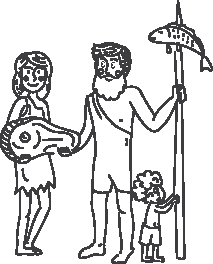
\includegraphics[scale=1.3]{willpower/ch2/1.pdf}
  
\includegraphics[scale=1.3]{willpower/ch2/2.pdf}    
\end{figure}

За сотні гадоў мы прыйшлі ад голаду ды інфэкцыяў да багатага харчаваньня і стэрыльнай чысьціні, але сталі пакутаваць на «хваробы цывілізацыі», якія рэдкія ў~паляўнічых-зьбіральнікаў сучаснай Афрыкі і Паўднёвай Амэрыкі, але часта сустракаюцца ў~прадстаўнікоў «цывілізаванага сьвету». Так, мы жывём больш, але й больш пакутуем ад розных неінфэкцыйных захворваньняў, што значна пагаршаюць якасьць нашага паўсядзённага жыцьця.

Паводле розных ацэнак, 90--100 тысячаў гадоў прадстаўнікі віду Homo sapiens вялі лад жыцьця паляўнічых-зьбіральнікаў, і толькі апошнія 5--6 тысячаў гадоў пачала разьвівацца цывілізацыя. Нашы гены прыстасаваліся да пэўнага асяродзьдзя, мы да яго былі цалкам адаптаваны. Пры рэзкіх зьменах узьнікае неадпаведнасьць генаў і асяродзьдзя, нашыя гены не пасьпяваюць пераладавацца так хутка. Спрабуючы прыстасавацца да незвычайнага асяродзьдзя, арганізм шкодзіць сабе: нават адаптыўныя рэакцыі могуць аказацца разбуральнымі, а~цела і розум проста не пасьпяваюць за зьменамі.

Навакольнае асяродзьдзе пасылае нашаму целу шматлікія біялягічна важныя сыгналы. Зьмена асьветленасьці, колькасьць бактэрыяў, пагрозы і стрэс, ваганьні калярыйнасьці, тэмпэратура паветра, погляды навакольных~--- усё гэта ўплывае на тонкую настройку і рэгуляцыю нэрвовай, эндакрыннай ды імуннай сыстэмаў арганізму. Многія «паляпшэньні» сучаснасьці ігнаруюць нашу біялёгію: традыцыйна «хацелі як лепей, атрымалася як заўсёды». Цеплавы камфорт перакідаецца прыгнётам спаленьня тлушчу, перагрузка інфармацыяй і задавальненьнямі вядзе да дэпрэсіі, яркае сьвятло ў~любы час содняў разбурае сон. Усё гэта прыводзіць да зьніжэньня запасаў здароўя і павышэньня рызыкі захворваньняў. \textbf{Занадта шмат сьвятла, занадта шмат ежы, занадта шмат канапаў, занадта шмат працы~--- шкодна, таму хваробы цывілізацыі часта называюць і «хваробамі багацьця».}

\subsection*{Дэзадаптацыя}

Дзіўна, але прычыны многіх сёньняшніх захворваньняў у~мінулым былі эвалюцыйнымі адаптацыямі, што дапамагалі выжыць. Схільнасьць пераядаць цукар дапамагала нам зьесьці лішак садавіны і назапасіць тлушч, каб перажыць зіму, а~цяпер прыводзіць да дыябэту і атлусьценьня. Стрэсавае павышэньне ўзроўню глюкозы і тлушчаў у~крыві сілкавала нашы цягліцы, калі мы ўцякалі ад небясьпекі, а~цяпер выклікае атэрасклероз. Тыя гены, якія дапамагалі нам змагацца з~інфэкцыямі і паразытамі, узмацняючы запаленчую рэакцыю, прыводзяць да росту аўтаімунных і алергічных захворваньняў. Высокі ўзровень нявызначанасьці і стрэсу сёньня вядзе да таго, што мы пачынаем есьці больш і выбіраем ежу з~больш высокай калярыйнай шчыльнасьцю, але гэта не дапамагае нам выжыць. \textbf{Тое, што працавала ў~мінулым, сёньня аказваецца проста шкодным. Мы можам прыстасавацца да чаго заўгодна, але якую цану мы заплацім за адаптацыю?}

\textbf{Тэорыя эвалюцыйнай неадпаведнасьці пацьвярджае,} што многія нашы рэакцыі выпрацаваліся для адпаведнасьці іншаму асяродзьдзю, у~якім мы эвалюцыянавалі. Наш мозг і цела не прызначаныя для доўгага сядзеньня перад экранам, для сацыяльнай ізаляцыі, для перагрузкі ежай, для хранічнага стрэсу. Мэханізмы канфлікту «гены / асяродзьдзе» аднолькавыя для любых хваробаў цывілізацыі, таму ўсе яны вылечваюцца ў~межах адзінага падыходу. Да іх адносяцца ішэмічная хвароба сэрца, цукровы дыябэт 2 тыпу, атэрасклероз, гіпэртанія, інфаркты, інсульты, дэпрэсія, акнэ, гемарой, некаторыя пухліны, алергіі і аўтаімунныя захворваньні, бессань, астэахандроз, атлусьценьне і інш.

\begin{figure}[htb!]
  \centering
  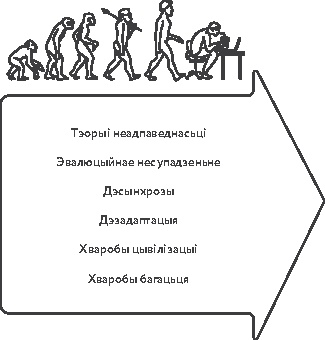
\includegraphics[scale=1.3]{willpower/ch2/3.pdf}
\end{figure}

\textbf{Напрыклад, у~мовах шматлікіх плямёнаў паляўнічых-зьбіральнікаў нават адсутнічаюць словы, якія абазначаюць бессань, а~падлеткі ніколі не сутыкаліся з~акнэ. Але варта перайсьці на заходні стыль харчаваньня, як тут жа зьяўляюцца высыпаньні.} Гэтыя хваробы дрэнна паддаюцца мэдыкамэнтознаму лячэньню. Сучасная мэдыцына не імкнецца вылечыць дыябэт 2 тыпу або гіпэртэнзію, а~можа толькі «кантраляваць іх». Пры атлусьценьні мэдыкамэнтозны эфэкт вельмі нязначны: напрыклад, за год лячэньня такімі прэпаратамі, як арлістат, страта вагі склала ўсяго 2,9 кг, сібутрамін~--- 4,7 кг. Пры гэтым у~«прэпаратаў ад пахуданьня» ёсьць сур'ёзныя пабочныя эфэкты і сындром адмены. Але ж, проста зьмяніўшы лад жыцьця, чалавек можа спакойна губляць 0,5--1 кг у~тыдзень.

Хваробы цывілізацыі забіваюць даволі павольна, але зьвязаныя з~заўчасным старэньнем, таму пагаршэньне здароўя прыводзіць да скарачэньня «маладога» часу жыцьця. Выяўляючы такія захворваньні на раньніх стадыях, можна запаволіць іх прагрэсаваньне, на позьніх жа стадыях зьмена ладу жыцьця ўжо не такая эфэктыўная.

\subsection*{Нэалітычная рэвалюцыя}

Першым прыкметным зьмяненьнем ладу жыцьця была нэалітычная рэвалюцыя (пачатак каля 9 тыс. гадоў да н.~э.), калі людзі перайшлі ад паляваньня і зьбіральніцтва да сельскай гаспадаркі. Гэты пераход ужо адбіўся ў~генах: людзі навучыліся спажываць малако, у~шматлікіх народаў павялічылася колькасьць копіяў фэрмэнту амілазы, што адказвае за страваваньне вугляводаў. Нягледзячы на тое, што нэалітычная рэвалюцыя прывяла да ўзьнікненьня першых цывілізацыяў, яе ўплыў на здароўе быў неадназначны.

\emph{Пры раставаньні ледавікоў у~Альпах знайшлі цела чалавека, якое добра захавалася. Навукоўцы высьветлілі, што ён загінуў каля пяці тысячаў гадоў таму, і далі імя яму Этцы. Вывучэньне Этцы паказала, што ўжо тады людзі жылі далёка ня ў~райскай гармоніі з~прыродай. У яго былі паразытарныя інфэкцыі, якія ўзьнікаюць пры вядзеньні сельскай гаспадаркі, падвышанае ўтрыманьне мыш'яку і медзі ў~тканках як наступства заняткаў мэталургіяй, прыкметы атэрасклерозу і артрыту ў~45 гадоў, а~таксама прыкметы гвалту~--- зажылыя пераломы, наканечнік стрэлы ў~плячы, сьляды крыві іншых людзей на калчане са стрэламі.}

Скучанасьць у~больш буйных паселішчах, сумеснае пражываньне з~жывёламі, залежнасьць ад ураджаю, аднастайнасьць харчаваньня~--- усё гэта прывяло да таго, што здароўе людзей пагоршылася. Прыручэньне жывёлаў было прагрэсіўным крокам, але ад жывёлаў да нас перайшло мноства інфэкцый: адзёр, дыфтэрыя, грып. У нашы дні пашырэньне гаспадарчых тэрыторый таксама павялічвае рызыку такіх пераходаў, як і ў~выпадку каранавіруснай інфэкцыі. Высокая шчыльнасьць насельніцтва добрая тым, што спрыяе гандлю і разьвіцьцю культуры, але рызыка яе ў~тым, што яна зьяўляецца асяродзьдзем для распаўсюду эпідэміяў. А вось ва ўмовах нізкай шчыльнасьці насельніцтва эпідэміі проста немагчымыя.

Земляробы пачалі хварэць на карыес, у~іх стаў часьцей зьяўляцца дэфіцыт жалеза, зьнізілася спажываньне бялковай ежы. Расслаеньне прывяло да таго, што пэўныя сацыяльныя пласты пачалі пакутваць ад «хваробаў багацьця»: атлусьценьне, атэрасклероз, сардэчна-сасудзістыя хваробы зьяўляюцца ў~жрацоў і багатых людзей. Працаваць даводзілася больш, чым пры ранейшым ладзе жыцьця, што відаць з~пашкоджаньняў хрыбта: калі паляўнічы-зьбіральнік жыў ва ўмовах адноснага багацьця, дзе ён працаваў ня больш за 4 гадзіны, фэрмэр працаваў нашмат больш, а~рабочы індустрыяльнай эры~--- больш за 10--12 гадзінаў.

За апошнія некалькі тысячаў гадоў паменшыўся сярэдні рост людзей і аб'ём галаўнога мозгу. Мяркуючы па касьцяных парэштках, у~раньніх фэрмэраў паменшылася і працягласьць жыцьця.

\infobox{Ёсьць вэрсія, што пераход да сельскай гаспадаркі быў прымусовы, а~ня добраахвотны. Прынамсі, сучасныя плямёны ня вельмі імкнуцца «цывілізавацца». Шмат хто ў~біблейскай гісторыі выгнаньня з~Раю~--- «У поце твару твайго будзеш есьці хлеб»~--- бачаць водгульле гісторый аб пераходзе да сельскай гаспадаркі.}

Лад жыцьця~--- гэта суплёт розных складнікаў, і асобныя яго кампанэнты ўносяць свой уклад у~разьвіцьцё хваробаў цывілізацыі. Напрыклад, калі ўзяць артэрыяльную гіпэртэнзію, то яе рызыка павялічваецца пры высокім спажываньні солі (а наш арганізм адаптаваны, хутчэй, да дэфіцыту натрыю, чым да лішку, затрымка натрыю павялічвае ціск), пры высокім узроўні хранічнага стрэсу, нізкай рухальнай актыўнасьці, калі ў~сасудах выпрацоўваецца менш сасудапашыральнага рэчыва аксіду азоту. Гэтыя фактары могуць спалучацца: так, пры высокім узроўні стрэсу чалавек менш рухаецца і есьць больш паўфабрыкатаў.

\subsection*{Першая эпідэміялягічная рэвалюцыя}

Эпідэміялягічны пераход~--- гэта рэзкае зьніжэньне колькасьці сьмерцяў ад эпідэмій, голаду, інфэкцыяў і атручэньняў, зьніжэньне дзіцячай сьмяротнасьці. Прычынамі сьмерці становяцца ўнутраныя, «дэгенэратыўныя», то бок хваробы, зьвязаныя са старэньнем, або прычыны, зьвязаныя з~самім чалавекам, напрыклад траўмы ці суіцыд.

З канца XVIII стагодзьдзя ў~Еўропе ўпершыню за тысячу гадоў пачаўся рост сярэдняй працягласьці жыцьця~--- яна перавысіла 40 гадоў. Магчыма, гэта было зьвязана з~сацыяльнымі зьменамі~--- распадам фэадальнага грамадзтва, паступовым зьяўленьнем сярэдняга класа і фармаваньнем грамадзкіх інстытутаў, якія ставілі здароўе насельніцтва ў~прыярытэт. Паляпшэньне санітарных умоваў і якасьці харчаваньня, рост прыбыткаў, павышэньне ўзроўню адукацыі, разуменьне прычынаў узьнікненьня інфэкцыяў ды іх прафіляктыкі~--- усе гэтыя фактары адыгралі сваю важную ролю. Адкрыцьцё сульфаніламідаў і антыбіётыкаў дазваляла ўзяць пад кантроль лячэньне сухотаў. На рубяжы ХІХ--ХХ стагодзьдзяў сярэдняя працягласьць жыцьця перавысіла 60 гадоў.

\subsection*{Другая эпідэміялягічная рэвалюцыя}

Аднак у~50--60-х гадах мінулага стагодзьдзя намецілася запаволеньне росту працягласьці жыцьця, а~ў некаторых краінах назіраўся рост сьмяротнасьці ад сардэчна-сасудзістых хваробаў. Новы этап зьніжэньня сьмяротнасьці быў зьвязаны з~заўважным павелічэньнем выдаткаў на сыстэму аховы здароўя. Узмацнілася ахова навакольнага асяродзьдзя, кантроль бясьпекі на вытворчасьці, распаўсюдзіліся дыспансеэрызацыя і прапаганда здаровага ладу жыцьця. Узровень дабрабыту людзей падвышаўся, здаровы лад жыцьця стаў модным. У канцы 60-х~--- пачатку 70-х адбыўся новы ўсплёск паляпшэньня жыцьця і паказьнікаў здароўя.

\emph{На жаль, пры моцных крызісах можа адбывацца і адваротны эпідэміялягічны пераход: рост сьмяротнасьці, павелічэньне колькасьці інфэкцыяў, зьніжэньне працягласьці жыцьця. Асабліва яскрава гэта выявілася, напрыклад, у~90-я гады ў~шматлікіх постсавецкіх краінах.}

На этапе другой эпідэміялягічнай рэвалюцыі галоўная задача мэдыцыны~--- падоўжыць жыцьцё і абараніць ад перадухільных захворваньняў. Чаргою ідуць сардэчна-сасудзістыя захворваньні (ССЗ), затым пухліны, затым нэўрадэгенэратыўныя хваробы. У сьвеце цяпер менавіта ССЗ~--- галоўны чыньнік інваліднасьці і сьмяротнасьці, і гэта можна эфэктыўна зьмяншаць раньняй дыягностыкай, ужо наяўнымі ў~арсэнале мэдыцыны сродкамі, а~таксама зьменай ладу жыцьця. Важным застаецца і зьніжэньне сьмяротнасьці ад вонкавых прычынаў сьмерці, сюды адносяцца аварыі, траўмы, суіцыды, атручэньні, перадазіроўка наркотыкамі і да т.~п. У нашыя дні гэта вядучая прычына сьмерці ва ўзросьце да 35 гадоў.

\infobox{У разьвітых краінах з~высокім узроўнем даходу асноўнай прычынай сьмерці становяцца анкалягічныя захворваньні, а~не сардэчна-сасудзістыя, як было раней. Пры гэтым працягласьць жыцьця павялічылася да 80 і больш гадоў.}

«Усе мы паміраем ад раку, але ня ўсе да яго дажываем»,~--- ёсьць такі жарт у~патолягаанатамаў. Цяпер мы назіраем фундаментальны зрух у~лячэньні анкалягічных захворваньняў, асновы якога закладзеныя дастаткова даўно ў~выглядзе праграм фінансаваньня навуковых дасьледаваньняў: зьяўляюцца новыя мэтады імунатэрапіі, да кожнай пухліны распрацоўваецца індывідуальны падыход з~генатыпаваньнем. У бліжэйшыя гады мы чакаем прагрэс у~лячэньні ўсё новых відаў раку.

Але, пераадолеўшы гэтыя сьмяротныя захворваньні, важна захоўваць ясны розум, энэргічнасьць і жаданьне жыць да канца сваіх дзён. Вырашаць пытаньні менавіта здаровага даўгалецьця, бо павелічэньне працягласьці жыцьця прыводзіць да павелічэньня пэрыяду хваробаў. На жаль, посьпех у~лячэньні нэўрадэгенэратыўных захворваньняў пакуль больш чым сьціплы: апошнім часам правалілася вялікая колькасьць патэнцыйных прэпаратаў ад хваробы Альцгаймэра. Аднак зьмена ладу жыцьця дазваляе істотна паўплываць на перадухіленьне і запаволіць разьвіцьцё нэўрадэгенэратыўных захворваньняў. 

\emph{Для мяне асабіста гэта вельмі актуальная тэма: генэтычны тэст паказаў, што я носьбіт мутацыі і схільны да ўзьнікненьня хваробы Альцгаймэра.}

\subsection*{Трэцяя эпідэміялягічная рэвалюцыя}

Як жартуюць мае калегі: «Здароўе~--- гэта магчымасьць памерці самым павольным з~усіх спосабаў». Узроставыя дэгенэратыўныя захворваньні можна ўявіць у~выглядзе зьедлівага дыму, тады як крыніцай яго зьяўляецца полымя~--- старэньне.

Ня мае сэнсу разганяць дым, мяняць мадэлі рэсьпіратараў або затрымліваць паветра~--- сьмерць непазьбежная. У навуковых колах ужо зьявілася разуменьне і ўпэўненасьць у~тым, што менавіта старэньне~--- корань усіх узроставых хваробаў. Ня мае сэнсу лячыць іх паасобку, таму важна сфакусавацца на самай галоўнай задачы~--- барацьбе са старэньнем.

Старэньне~--- такі ж фізыялягічны мэханізм, як і ўсе астатнія, таму нам варта перастаць адчуваць трапятаньне і містычную пакору перад гэтым працэсам, трэ ўкладваць сродкі ў~фундамэнтальныя навукі для вывучэньня мэтабалічных, гарманальных, генэтычных, малекулярных заканамернасьцяў старэньня.

Навука старэньня атрымлівае вельмі мала фінансаваньня ў~параўнаньні зь іншымі галінамі. Людзі паводзяцца так, як быццам жывуць вечна, а~старэць і паміраць будзе нехта іншы, але не яны. Ёсьць у~гэтым, магчыма, і матэрыяльныя аспэкты: «Для фармы anti-age лекі як электрамабіль для нафтавікоў». Бо эфэктыўная антыўзроставая тэрапія зробіць непатрэбнымі большасьць прэпаратаў для лячэньня шматлікіх захворваньняў. Скажыце сабе, маўляў, жыву не чацьвёрты дзясятак, а~ўсяго толькі першую сотню!


\subsection*{Пытаньні і заданьні}

1. На што цяпер хварэюць і ад чаго паміраюць людзі ў~вашым асяродзьдзі?

2. Якіх хваробаў вы асьцерагаецеся больш за ўсё?

3. Як бы вы хацелі пачувацца ў~старасьці?


\section{Эвалюцыя і здароўе}

«Нішто ў~біялёгіі ня мае сэнсу, апроч як у~сьвятле эвалюцыі»,~--- заўважыў генэтык-эвалюцыяніст Феадосій Дабржанскі. Я люблю разблытваць складаныя эвалюцыйныя мэханізмы, бо яны могуць шмат расказаць пра тое, чаму мы сябе паводзім і адчуваем сёньня менавіта так, а~не інакш. Многія асаблівасьці нашых паводзінаў эвалюцыйна абумоўленыя, а~веданьне гэтага дапаможа нам лепей разумець сябе.

Калі мы глядзім у~каламутную глыбіню гісторыі, можам убачыць два супярэчлівыя погляды. З аднаго боку, ёсьць вэрсія аб тым, як моцна мардаваліся й пакутавалі нашыя продкі паляўнічыя-зьбіральнікі ў~каменным веку, як, ледзь дасягнуўшы палавой сталасьці, гінулі ад драпежнікаў ці інфэкцыі, а~ўсё сваё нядоўгае жыцьцё праводзілі ў~цяжкай працы. Іншы погляд кажа пра «залатое стагодзьдзе», калі нашы продкі жылі ў~асяродзьдзі, цалкам адптаваным пад іх гены. Качавы лад жыцьця і багацьце рэсурсаў дазвалялі паляўнічым-зьбіральнікам працаваць некалькі гадзінаў у~дзень, хоць з~разьвіцьцём нашай цывілізацыі мы сталі працаваць усё больш. Вонкавы выгляд сучасных паляўнічых-зьбіральнікаў, худых і мускулістых, кажа на іх карысьць, у~параўнаньні са слабымі і поўнымі жыхарамі мэгаполісаў.

Зьвесткі аб працягласьці жыцьця і прычынах сьмерці людзей у~розныя гістарычныя часы дакладна ўстанавіць немагчыма, у~кожным выпадку сярэдняя працягласьць жыцьця была невысокай~--- як праз высокую дзіцячую сьмяротнасьць, так і з~прычыны міжпляменных сутыкненьняў. У каменным веку ўзровень агрэсіі быў, імаверна, вельмі высокі. Нам можа здавацца, што мы жывём у~небясьпечны час, але сьвет становіцца ўсё больш цывілізаваным, ды й злачыннасьць у~апошнія дзесяцігодзьдзі зьмяншаецца. А бо ў~паляўнічых-зьбіральнікаў гвалтоўная сьмерць была адной з~самых распаўсюджаных, плямёны ўвесь час ваявалі міжсобку. 

\emph{Нават у~нашы дні ў~індзейцаў янамама ў~Амазоніі ад міжпляменных звадак гіне каля траціны маладых мужчынаў, прычым гэтая схільнасьць «бі чужых» назіраецца ўжо на працягу некалькіх пакаленьняў.}

\subsection*{Цана адаптацыі}

Культурныя зьмены ў~гісторыі нашай цывілізацыі суправаджаліся драматычнай зьменай і здароўя, і вонкавага выгляду людзей. Напрыклад, засяляючы паўночныя тэрыторыі, людзі сутыкнуліся з~дэфіцытам вітаміну D. Пад узьдзеяньнем натуральнага адбору перавагу атрымалі сьветлыя адценьні скуры, якія дазвалялі забясьпечваць аптымальны ўзровень гэтага вітаміну і пры меншай сонечнай актыўнасьці. 

Саграваючыся ў~зямлянках і дамах агменем без вывадной трубы, нашы продкі дыхалі вялікай колькасьцю дыму, што вельмі шкодна ўплывала на здароўе, павялічваючы рызыку хваробаў сэрца і раку лёгкіх. Магчыма, гэта прыносіла шкоду яшчэ большую, чым паветра сучасных загазаваных гарадоў.

\textbf{Працягласьць жыцьця} людзей шмат у~чым павялічылася дзякуючы чыстай вадзе і якаснай ежы ў~дастатковай колькасьці. Цяпер усё радзей можна сутыкнуцца з~дэфіцытам калёрыяў, але пры гэтым разнастайнасьць нашай ежы значна зьнізілася. Большасьць людзей есьць меней за 20 тыпаў ежы і часьцей за ўсё ў~рафінаваным выглядзе: з~пшаніцы, соі, мяса і рысу. Для параўнаньня~--- старажытныя елі абсалютна ўсё, і гэта было каля 1000 найменьняў расьліннай і жывёльнай ежы. Бывае так, што занадта «правільны» лад жыцьця можа прывесьці да фармаваньня сур'ёзных дэфіцытаў. Напрыклад, адмаўляючыся ад гатовай ежы, солі, морапрадуктаў, можна атрымаць дэфіцыт ёду, калі жывеш у~раёнах зь яго нізкім утрыманьнем.

\subsection*{Занадта чыста} 

Чысьціня выратавала нас ад шматлікіх інфэкцыяў, але павялічыла колькасьць алергій і аўтаімунных захворваньняў. Чым чысьцейшае асяродзьдзе, чым актыўнейшае ўжываньне антыбіётыкаў, тым меншая разнастайнасьць мікрафлёры кішачніка, што правакуе мноства парушэньняў здароўя. Рост гэтых захворваньняў настолькі вялікі, што гаворка ідзе ўжо пра эпідэмію аўтаімунных захворваньняў. Сучасны жыхар страціў ужо палову відаў мікробаў, пры гэтым нарастае прапорцыя шкодных і зьмяншаецца частка карысных бактэрыяў.

\begin{figure*}[htb!]
  \centering
  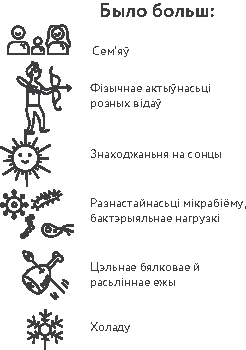
\includegraphics[align=t,scale=1.5]{willpower/ch2/4.pdf}\qquad\qquad
  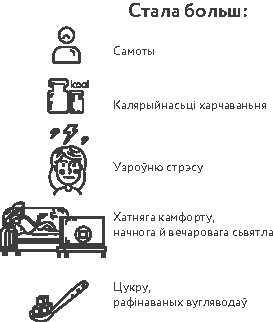
\includegraphics[align=t,scale=1.5]{willpower/ch2/5.pdf}
\end{figure*}

\subsection*{Мала руху}

З кожным дзесяцігодзьдзем мы ўсё меней рухаемся, а~разьвіцьцё службы даставак робіць выйсьце з~дому зусім не абавязковым. Доля фізычнае працы сёньня ўпала з~94 адсоткаў да 4 адсоткаў. 

\emph{Калі мы параўнаем чалавека з~племя хадза, што жыве ў~Танзаніі, зь любым гараджанінам, то хадза ў~14 раз больш рухаецца, прычым гаворка ідзе пра паўсядзённыя актыўнасьці: хада, зьмена паставы, сядзеньне на кукішках, а~не на крэсьле, і да т.~п. Такая рухальная актыўнасьць у~першую чаргу важная для сардэчна-сасудзістага здароўя: любы рух спрыяе выпрацоўцы аксіду азоту, які зьніжае ціск і важны для нашых сасудаў і сэрца. У племені хадза пажылыя людзі з~артэрыяльным ціскам 160 і вышэй зьяўляюцца рэдкасьцю. А менавіта гіпэртэнзія запускае шматлікія іншыя хваробы сэрца.}

Частай праблемай зьяўляюцца і хваробы «недавыкарыстаньня», такія як астэапароз, які сустракаецца ў~кожнай трэцяй жанчыны пасьля 50 гадоў. Калі мы маем мала фізычнае актыўнасьці, то і маса касьцей у~нас меншая. Тыя людзі, якія меней рухаюцца, ужо ў~дзяцінстве маюць меншую цяглічную масу, якая пры старэньні пачынае памяншацца, ведучы да астэапарозу і яго наступстваў, такім як пераломы шыйкі сьцягна, кампрэсійныя пераломы хрыбта.

Да ліку хваробаў недакарыстаньня адносіцца і саркапэнія (страта цяглічнай масы), якая пачынаецца ўжо з~30 гадоў, а~таксама плоскаступнёвасьць (наступства нашэньня нязручнага абутку і дэфармацыі стопаў), парушэньне прыкусу (дэфіцыт цьвёрдай ежы, занадта мяккая ежа). А вось жаваньне спрыяе і падтрыманьню здароўя зубоў, і разьвіцьцю больш актыўнай мімікі. Таксама частай праблемай зьяўляюцца болі ў~паясьніцы. Працяглае сядзеньне вядзе да паслабленьня цягліцаў сьпіны, скарачэньню паясьнічнай цягліцы і да гіпэрлардозу. Слабая паясьніца можа пашкодзіцца нават ад невялікай нагрузкі.

\emph{Тыя людзі, у~каго дастаткова фізычнае актыўнасьці, нашмат радзей сутыкаюцца з~праблемай боляў у~сьпіне. У некаторых маіх кліентаў пазьбяганьне паясьнічнага болю ледзь не асноўная матывацыя да заняткаў спортам. Хранічны стрэс таксама можа выклікаць цяглічную напругу і павялічыць рызыку траўмаў, таму й псыхасацыяльныя чыньнікі павялічваюць рызыку боляў у~паясьніцы.}

\subsection*{Болей стрэсу}

У нас стала больш даступнай інфармацыі, больш магчымасьцяў, больш мабільнасьці~--- і гэта выдатна. Але разам з~тым узрасьлі інфармацыйная перагрузка, стрэс, нявызначанасьць. Хуткасьць зьменаў у~сьвеце такая высокая, што псыхіка чалавека не пасьпявае адаптавацца. Стала менш гострага стрэсу, але нашмат больш дэпрэсій. Ды і ў~цэлым становіцца занадта шмат усяго: калёрыяў, стымуляцыі, шуму, сьвятла, якія зьбіваюць нашыя ўнутраныя гадзіньнікі. Наўрад ці рэгулярнае начное няспаньне было папулярнае пры адсутнасьці электрычнага асьвятленьня.

\subsection*{Болей нявызначанасьці}

Ранейшыя каштоўнасьці, традыцыі, сацыяльныя інстытуты старэюць і перастаюць задавальняць людзей. Старыя ўстаноўкі разбураныя, а~новых матывацыяў пакуль ня створана, што вядзе да крызісу сэнсу. Кагосьці падтрымлівае вера ў~бога, якая зьяўляецца свайго кшталту абаронай, памяншаючы імавернасьць дэпрэсіі. Тым ня менш кожны чалавек у~нашым цывілізаваным сьвеце стаіць перад задачай усьведамленьня і стварэньня сваёй ідэнтычнасьці. Сем'і распадаюцца, усё больш людзей жывуць самотна, а~частата асабістых кантактаў памяншаецца. \textbf{Усё гэта ўзмацняе разьяднанасьць, сацыяльную ізаляцыю і павялічвае рызыкі для здароўя.}

\subsection*{Эфэкт бабулі}

Дасьледаваньне мэтрычных кніг дазволіла матэматычна давесьці «правіла бабулі». Пажылыя жанчыны атульваюць клопатам уласных унукаў, пакуль іх дзеці занятыя сваімі справамі. А значыць, дапамагаюць нейкім сваім генам зацьвердзіцца ў~наступным пакаленьні. Калі ёсьць магчымасьць «пакінуць дзіця на бабулю», можна нарадзіць і другое, і трэцяе. А мэнапаўза патрэбная для таго, каб прымірыць эвалюцыйна-генэтычныя інтарэсы розных бацькоўскіх пакаленьняў. Высокая працягласьць жыцьця жанчынаў пасьля мэнапаўзы замацавалася генэтычна, каб падоўжыць жыцьцё ўсім нам. Устаноўлена, што наяўнасьць бабулі па кудзелі скарачае рызыку дзіцячай сьмяротнасьці напалову. Акрамя таго, дзеці, зь якімі займаліся бабулі, стабільна дэманструюць лепшыя паказьнікі разумовага разьвіцьця.

\subsection*{Пытаньні і заданьні}

1. Ці карыстаецеся вы антыбактэрыйным мылам? Ці выкарыстоўваеце сродкі дэзынфэкцыі для ўборкі і мыцьця?

2. Ці пачалі вы карыстацца службамі дастаўкі замест паходу ў~краму?

3. Пагаварыце са сваімі бацькамі, бабулямі і дзядулямі пра стрэс, рух, ежу, чысьціню ў~іх час і параўнайце з~сучаснасьцю.


\section{Як хваробы багатых сталі хваробамі бедных}

Даўно заўважана, што пэўны лад жыцьця зьвязаны са здароўем і з~тым, на што хварэюць людзі. З нарастаньнем няроўнасьці ў~грамадзтве зьявіліся «хваробы багатых» і «хваробы бедных». А рэзкія зьмены ў~культуры здароўя за апошнія дзесяцігодзьдзі прывялі да таго, што «багатыя» і «бедныя» памяняліся месцамі: цяпер ужо бедныя людзі пераважна маюць «хваробы багатых». Гучыць заблытана? Давайце разьбяром гэта на прыкладах.

\subsection*{Атлусьценьне}

Такім чынам, заможныя людзі са старажытных часоў мелі доступ да лішку ежы, прычым да найболей калярыйнай ежы: болей тлушчу, мёду, алькаголю, мяса, мукі. Пры гэтым яны мала рухаліся, праводзячы шмат часу ў~закрытых памяшканьнях. Гучыць падобна да жыцьця сучаснага чалавека? Нядзіўна, што ў~такіх людзей часьцей разьвіваліся такія вядомыя нам захворваньні «ладу жыцьця». На тле нездаровага харчаваньня, маларухомасьці, нястрыманасьці гэтыя хваробы ўзьнікалі і тысячы, і сотні гадоў таму.

Дасьледаваньне муміі старажытнаэгіпецкай царыцы Хатшэпсут паказала, што яна хварэла на дыябэт, у~яе было выразнае атлусьценьне, а~таксама моцны карыес, які ўскладніўся зубным абсцэсам. Зрэшты, і тады, і цяпер атлусьценьне спрабавалі схаваць, статуі й выявы царыцы паказваюць нам яе досыць падцягнутай. Адыліж пасьля 30 гадоў кіраваньня фараон павінен быў кожныя тры гады па коле абабягаць свой палац, паказваючы сілу і здольнасьць кіраваць далей!

\emph{«Патураць целу, даваць яму лішняе, звыш таго, што яму трэба,~--- вялікая памылка ўжо таму, што ад раскошнага жыцьця не дадаецца, а~памяншаецца задавальненьне ад ежы, адпачынку, ад сну, ад адзеньня, ад памяшканьня. Стаў есьці лішняе, салодкае, не прагаладаўшыся, разладжваецца страўнік, і няма ахвоты да ежы і задавальненьняў.}

\emph{Стаў езьдзіць там, дзе мог пешшу прайсьці, звык да мяккай пасьцелі, да далікатнай, салодкай ежы, да раскошнага ўбранства ў~доме, звык прымушаць рабіць іншых, што сам можаш зрабіць ,~--- і няма радасьці адпачынку пасьля працы, цяпла пасьля холаду, няма моцнага сну і ўсё больш аслабляеш сябе і не дадаеш, а~зьмяншаеш радасьці і спакою і свабоды»,~--- вялікі класік Леў Талстой ведаў, пра што кажа, пішучы ў~1910 годзе свой «Шлях жыцьця».}

\infobox{Многія «хваробы цывілізацыі», распаўсюджаныя сёньня,~--- алергіі, атлусьценьне, дыябэт, дэпрэсія,~--- у~старажытнасьці былі толькі ў~некаторых людзей з~высокім сацыяльным статусам, прыбыткам і адпаведным няўстрыманым ладам жыцьця.} 

Некаторымі хваробамі нават ганарыліся, лічачы іх прыкметай вытанчанасьці. Так, падагру называлі «хваробай каралёў», бо толькі багатым людзям была даступная вялікая колькасьць бялковай ежы і алькаголю на працягу доўгага часу ў~спалучэньні з~маларухомым ладам жыцьця.

Атлусьценьне лічылася сымбалем статусу, некаторыя плямёны спэцыяльна адкормлівалі дзяўчат, каб пасьпяхова выдаць іх замуж. І калі раней нявесты ад'ядаліся перад вясельлем, каб зрабіць уражаньне, сёньня яны худнеюць роўна дзеля гэтага ж. У мінулым людзі выраблялі фігуркі вельмі поўных жанчынаў як магчымы аб'ект пакланеньня, а~цяпер залішняя вага выклікае не захапленьне, а~шкадаваньне. У наш час у~бедных краінах атлусьценьне сустракаецца часьцей сярод заможных людзей, а~вось у~багатых краінах~--- сярод бедных, бо людзі з~высокім статусам і прыбыткам маюць час, сродкі і жаданьне займацца сваім здароўем.

\emph{Цяпер траціна жыхароў плянэты пакутуе ад лішняй вагі. Атлусьценьне павышае рызыку дыябэту, сардэчна-сасудзістых захворваньняў, многіх відаў раку і кароціць жыцьцё ў~сярэднім на 5--15 гадоў. Кожная пятая сьмерць у~сьвеце адбываецца з~прычыны залішняй вагі.}

\subsection*{Псыхічныя разлады}

Старажытнагрэцкі філёзаф Арыстотэль задаваў пытаньне: «Чаму людзі, якія зьзялі талентам у~галіне філязофіі, або ў~кіраваньні дзяржавай, або ў~паэтычнай творчасьці, або ў~занятках мастацтвам,~--- чаму ўсе яны, відаць, былі мэлянхолікамі?» Геракл, які шанаваўся ў~старажытных грэкаў і як герой, і як бог, пакутаваў на «разьліцьцё чорнай жоўці»~--- а~менавіта на мэлянхолію.

\emph{«Багаты ангелец ад нуды падарожнічае, ад нуды робіцца паляўнічым, ад нуды матае, ад нуды жэніцца, ад нуды страляецца»,~--- так апісваў у~канцы XVIII стагодзьдзя ў~«Лістах рускага падарожніка» Мікалай Карамзін цэнтар спліну й мэлянхоліі~--- Брытанскую імпэрыю.}

\subsection*{Эпідэмія роспачы і безнадзейнасьці} 

У наш час павелічэньне сацыяльнай няроўнасьці, зьніжэньне заробкаў, павелічэньне стрэсу суправаджаюцца і стратай сацыяльнай падтрымкі ад сваякоў і сяброў, нарастаньнем ізаляцыі, крызісам каштоўнасьцяў і сэнсаў. Гэта прыводзіць да росту колькасьці суіцыдаў, колькасьці сьмерцяў ад перадазіроўкі наркотыкамі, алькаголем. У наш час ад самагубстваў гіне больш людзей, чым ад войнаў, забойстваў, тэрактаў разам узятых. У постсавецкіх краінах узровень суіцыду ў~тры разы вышэйшы за сусьветны. Перадазіроўка наркотыкамі ў~ЗША забірае больш жыцьцяў, чым аўтакатастрофы. Маладыя людзі часьцей гінуць ад суіцыду, алькагольнай хваробы печані і перадазіроўкі, і гэта вядзе да прыкметнага павелічэньня сьмяротнасьці.

\subsection*{Эпідэмія залежнасьцяў} 

Людзі з~даўніх часоў зь цікаўнасьцю цягнуліся да рэчываў, якія зьмяняюць стан сьвядомасьці. Расьліны ўтрымліваюць псыхаактыўныя рэчывы ў~невялікіх колькасьцях і не выклікаюць моцнай залежнасьці. Але ўсё зьмянілася ў~апошняе стагодзьдзе, калі стала магчыма вырабляць магутныя наркотыкі ў~высокіх канцэнтрацыях і выкарыстоўваць іх нутрывэнна. Сталі таннымі й даступнымі і «легальныя» наркотыкі, такія як нікатын і алькаголь. Шырока распаўсюдзіліся казіно, латарэі, што выклікаюць залежнасьць, стала больш бясплатнага порна.

Празьмернасьць стымуляцыі можа выклікаць залежнасьці і прыводзіць да парушэньня рэгуляцыі дафамінавых рэцэптараў. Занадта моцная стымуляцыя вядзе да разьвіцьця \textbf{«сындрому дэфіцыту задаволенасьці»}, калі чалавек страчвае здольнасьць атрымліваць задавальненьне ад паўсядзённых рэчаў і змушаны зьвяртацца да звышстымулаў. Напрыклад, ёсьць вялікая розьніца паміж эратычнымі фантазіямі ды інтэрнэт-порна ў~высокім разрозьненьні. Чым болей вы гледзіце порна, тым мацней абясцэньваеце партнёра, меней атрымліваеце задавальненьня ад «нармальнага» сэксу, павялічваецца рызыка эрэктыльнай дысфункцыі.

\emph{Распаўсюджваньне наркотыкаў набывае характар эпідэміі, усё больш дзяцей уцягваюцца ў~залежнасьць. З 2000 па 2015 год колькасьць сьмерцяў, зьвязаных з~наркотыкамі, вырасла на 60\,\%. Пры гэтым эфэктыўнасьць лячэньня наркаманіі вельмі нізкая, каля 5\,\%. Наркаманы зьдзяйсьняюць велізарную колькасьць злачынстваў, уцягваюць у~наркаспажываньне іншых людзей. Сусьветны наркатрафік перавышае 800 мільярдаў даляраў, і траціна гэтай сумы ідзе на подкуп чыноўнікаў і паліцыі. Падзел на «лёгкія» і «цяжкія» наркотыкі такі ж падманлівы, як «лёгкія» і «цяжкія» цыгарэты, бо 80\,\% цяжкіх наркаманаў пачыналі менавіта зь «лёгкіх» наркотыкаў. Многія лекавыя сродкі могуць быць наўмысна выкарыстаны як наркотыкі, што прыводзіць да разбуральных наступстваў, як было падчас «апіятнай катастрофы» ў~ЗША.}

\subsection*{Адыктыўная дэфармацыя асобы}

Наркаманія найбольш небясьпечная таму, што разбурае асобу. Напрыклад, какаін можа выклікаць устойлівую дэфармацыю («рубец асобы») нават за некалькі месяцаў прымяненьня, хутчэй, чым любыя іншыя віды наркотыкаў. У адрозьненьне ад іншых сымптомаў залежнасьці, зьмены асобы могуць быць незваротнымі або цяжказваротнымі. Асноўныя прыкметы наркатычнай дэфармацыі асобы: непазьбежнае фармаваньне дэпрэсіі, зьбядненьне спэктру эмацыйных рэакцыяў, страта здольнасьці адрозьніваць дэталі, пастаянныя перапады настрою, ілжывае адчуваньне ўласнае велічы, самаўпэўненасьць, нахабства. Людзі атрымліваюць «здольнасьць» вельмі пераканаўча хлусіць (эмацыйнае прытупленьне робіць хлусьню больш пераканаўчай), падае крытычнае стаўленьне да свайго стану, часта нават без ужываньня захоўваюцца ідэі перасьледу, значна зьніжаюцца маральна-этычныя нормы і правілы.

\subsection*{Алькагалізм} 

Нядаўна на кансультацыі я пачуў дзіўнае пытаньне: «Скажыце, ці абавязкова піць віно, а~то я ад яго ня вельмі добра пачуваюся». Высьветлілася, што для многіх людзей, якія цікавяцца здароўем, келіх віна практычна прыраўняўся да мэдытацыі або прысяданьняў, а~адмова ад яго бачыцца нейкім нездаровым рашэньнем. Нехта тлумачыць гэта карыснымі рэсвэратролам (антыаксыдант~--- \emph{заўв.}) у~складзе, хтосьці~--- «антыстрэсавымі малымі дозамі» і да т.~п. Навуковыя дасьледаваньні паказваюць, што, незалежна ад прычыны сьмерці, верагоднасьць сьмерці залежыць ад выпітага алькаголю. Сувязь, вядома, нелінейная, але жыцьцё скарачаецца нават пры мінімальным узроўні спажываньня~--- менш за 100 мл сьпірту (то бок менш чым бутэлька віна ў~тыдзень). Такое мінімальнае спажываньне скарачае жыцьцё на паўгода к 40 гадам, а~пры ўзроўні спажываньня вышэй за 350 мл сьпірту~--- на пяць гадоў.

\infobox{Нягледзячы на некаторыя факты так званага «пазітыўнага ўплыву» алькаголю на арганізм, няма навуковых зьвестак аб яго станоўчым узьдзеяньні ў~доўгатэрміновай пэрспэктыве.}

Для любога шкоднага фактару існуюць дзьве групы рызыкаў: дэтэрмінаваныя (залежныя ад дозы) і стахастычныя (бяз дозавага парога). У аснове прыведзеных навуковых «бясьпечных» дозаў алькаголю~--- яго ўзьдзеяньне на печань. Тут усё зразумела: чым больш п'е чалавек, тым горш ягонай печані. Але існуе мноства станаў і сытуацый, калі нават малыя дозы маюць вялікае значэньне. Сюды ўваходзяць сацыяльныя рызыкі, траўмы, заганы разьвіцьця плода і рызыкі павышэньня імавернасьці іншых захворваньняў (дэпрэсія, шызафрэнія, рак, парушэньне рытму сэрца і інш.). Праўда ў~тым, што алькаголь можа прычыніць шкоду мноствам разнастайных спосабаў, бо існуе 30 захворваньняў, якія выклікаюцца выключна алькаголем, і 200 хваробаў, узьнікненьню якіх ён актыўна спрыяе.

\emph{Алькаголь нават у~малых дозах павялічвае рызыку разьвіцьця раку: навукова даведзеная яго ўзаемасувязь з~ракам ротавай поласьці, носа, гартані, стрававода, тоўстай кішкі, печані і малочнай залозы ў~жанчынаў. Для гэтага дастаткова аднаго келіха віна ў~дзень. У цэлым ад 5 да 10\,\% ракавых захворваньняў могуць быць зьвязаныя з~ужываньнем алькаголю, а~памяншэньне яго спажываньня можа зьменшыць рызыку іх узьнікненьня. Ужываньне нават 10 грамаў сьпірту павялічвае рызыку парушэньня рытму сэрца.}

\textbf{Алькаголь~--- гэта адзіны наркотык, шкода ад якога для навакольных нават вышэйшая, чым для саміх пітакоў, зь ім часьцей за ўсё зьвязаныя рызыкоўныя і крымінальныя паводзіны.} Нават малыя дозы алькаголю прыгнятаюць работу вышэйшых цэнтраў кары галаўнога мозгу, што зьмяншае самакантроль і крытычнасьць. Так, у~стане алькагольнага ап'яненьня ўчыняецца больш за 80 адсоткаў забойстваў, выпадкаў цяжкіх цялесных пашкоджаньняў, згвалтаваньняў. Няма ніводнага ўнікальнага карыснага эфэкту этылавага сьпірту, акрамя яго ўнівэрсальнага разбуральнага дзеяньня.

\subsection*{Алергія}

Алергія першапачаткова таксама лічылася хваробай элітаў. Брытанскі лекар сэр Марэл Макензі ў~канцы XIX стагодзьдзя пісаў, што алергія~--- гэта «нагода для гонару, бо сянны катар паказвае на перавагу ва ўзроўні культуры і цывілізацыі ў~параўнаньні з~народамі, якім пашанцавала менш». Гэтая хвароба лічылася «моднай» і ў~сялянаў не назіралася.

Лекары тлумачылі алергію падвышанай «вытанчанасьцю, адчувальнасьцю, адукаванасьцю» і рэкамэндавалі для прафіляктыкі выкарыстоўваць какаін і тытунь у~спалучэньні з~горнымі курортамі ці сонечнымі марскімі выспамі \textbf{(не спрабуйце паўтарыць прынамсі першы «сьмяротны» нумар гэтай праграмы!)}.

\emph{Наогул магчымасьць весьці нездаровы лад жыцьця лічылася прэстыжнай. Хадзіць пешшу!? Не, гэта~--- прыкмета нізкага статусу. Таму арыстакратаў у~розных культурах насілі на насілках або ў~адмысловых паланкінах. Крэсла для рымлян~--- гэта паказьнік статусу: раб заўсёды насіў за чыноўнікам складаное, багата ўпрыгожанае крэсла. Рознага кшталту наркотыкі ды іншыя злоўжываньні ў~мінулым таксама былі прывілеем заможных людзей. У сучасным сьвеце схільнасьць курыць, піць і ўжываць дакладна ня будзе прыкметай статутнасьці, хутчэй наадварот.}

\subsection*{Хваробы праз дэфіцыт сонечнага сьвятла}

Загарэлы колер скуры лічыўся непрывабным, бо казаў пра тое, што чалавек працуе ў~полі. У тых, на каго працавалі і хто меў магчымасьць праводзіць больш часу ў~памяшканьні, скура была бялейшая. Таму ў~самых розных краінах жанчыны хаваліся ад сонца, выходзілі на вуліцу з~парасонамі і выкарыстоўвалі для адбельваньня небясьпечныя касмэтычныя сродкі, напрыклад валавяныя бялілы. Цяпер у~краінах Захаду ў~модзе ўмераны загар~--- прыкмета таго, што вам ня трэба сядзець у~офісе ўвесь час і ў~вас ёсьць магчымасьць адпачываць і прымаць сонечныя ванны. З пункту гледжаньня здароўя, вядома, карысна часьцей бываць на сонцы.

\subsection*{Пытаньні і заданьні}

1. Хто зь людзей вакол вас часьцей пакутуе на атлусьценьне? Што ў~іх агульнага?

2. Параўнайце лад жыцьця людзей з~высокім і нізкім узроўнем даходу ў~вашым асяродзьдзі. Якія асноўныя адрозьненьні ў~захворваньнях?

3. Ці шмат сярод вашых знаёмых людзей з~алергіямі? На што часьцей бывае алергія?


\section{Ежа багатых і бедных}

\subsection*{Цукар і мучныя вырабы}

Сёньня багатыя і адукаваныя людзі ядуць мала цукру і мучнога, шмат гародніны, больш цэльнай ежы. А малазабясьпечаныя ядуць шмат цукру, паўфабрыкатаў, мучнога і мала гародніны.

Спачатку многія высокакалярыйныя і ў~выніку небясьпечныя для здароўя прадукты былі даступныя толькі заможным людзям. Напрыклад, у~мінулым прасеяная белая мука, больш шкодная для здароўя, была па кішэні адно багацеям. Звычайныя людзі елі муку грубага памолу зь вялікай колькасьцю клятчаткі.

Цукар да XVI стагодзьдзя каштаваў вельмі дорага, у~XVIII стагодзьдзі яго спажывалі ня больш за кіляграм на чалавека ў~год. Цяпер яго ядуць у~50 разоў больш, прычым перадусім тыя людзі, хто харчуецца таннымі паўфабрыкатамі і ў~цэлым нездаровай ежай.

\subsection*{«Дыеты для бедных»}

Гістарычна многія дыеты, якія паказалі сваю карысьць для здароўя ў~навуковых дасьледаваньнях~--- напрыклад, міжземнаморская (крыцкая) або акінаўская дыета,~--- на паверку аказваюцца «дыетамі бедных». Недахоп прадуктаў харчаваньня «прымушаў» сялянаў уключаць у~рацыён вялікую разнастайнасьць расьлінных і жывёльных прадуктаў.

Напрыклад, у~крыцкай дыеце прысутнічае вялікая колькасьць зеляніны: на гэтай грэцкай высьпе гародніны ядуць у~некалькі разоў больш, чым у~кантынэнтальнай Эўропе. А вось чырвонага мяса~--- менш, бо мясцовыя жыхары строга трымаюць праваслаўныя пасты, якія могуць складаць ад 180 да 200 дзён у~годзе. Вінаградныя смаўжы ўвайшлі ў~францускую кухню з~часоў стогадовай вайны, калі сяляне елі што заўгодна, каб не памерці з~голаду. А цяпер гэтая страва лічыцца далікатэсам.

\subsection*{Травы}

Расьлінныя спэцыі карысныя, таму што памяншаюць колькасьць зьедзенага падчас прыёму ежы, добрыя для мікрафлёры, запавольваюць глікацыю, абараняюць прадукты пры тэрмічнай апрацоўцы, паляпшаюць ліпідны профіль, зьніжаюць актыўнасьць некаторых аксыдазаў (акісьляльных фэрмэнтаў) у~арганізьме чалавека і да т.~п. Цікава, што даданьне спэцый можа на 20\,\% зьменшыць уздым інсуліну пасьля прыёму ежы.

\emph{Магчыма, «францускі парадокс»~--- нізкае захворваньне сар\-дэч\-на-сасудзістымі хваробамі і нізкая сьмяротнасьць пры высокім спажываньні тлушчаў~--- зьвязаны з~актыўным ужываньнем спэцый, а~не віна: у~дзвюх чайных лыжках праванскіх траваў антыаксыдантаў больш, чым у~140 мл чырвонага віна або 40 грамах горкай чакаляды.}

Запомніце гэтыя назвы: размарын, базілік, чабор, шалвея, перцавая мята, арэгана, сатурэя садовая, маяран. І выкарыстоўвайце гэтыя травы пры гатаваньні. Сярод маіх асабістых фаварытаў цяпер размарын і арэгана. Іх плюс у~тым, што яны выдатна спалучаюцца з~усімі прадуктамі, няхай гэта будзе мяса, морапрадукты, гародніна ці салаты. Дадаваць можна сухую сумесь або папярэдне замочаную ў~аліўкавым алеі духмяную зеляніну.

\subsection*{Морапрадукты}

«Вустрыцы і галеча, падобна, заўсёды ідуць рука аб руку»,~--- пісаў у~свой час ангельскі раманіст Чарлз Дыкенс. Рыбакі называлі лобстараў «прусакамі мора» і нават выкідвалі іх, калі яны перапаўнялі сеткі й перашкаджалі лавіць рыбу. Тыя, у~каго бракавала грошай на мяса, надавалі шмат увагі дарам мора, а~ў далёкім мінулым дыета нашых прамых продкаў утрымлівала мноства морапрадуктаў, рыбы, водарасьцяў.

Некаторыя палеаантраполагі бачаць у~морапрадуктах ключ да эвалюцыі мозгу: рэчывы~--- ад ёду да Амега-3 кіслотаў, якія зьмяшчаюцца ў~іх у~высокіх канцэнтрацыях,~--- аказвалі стымулюючае ўзьдзеяньне на разьвіцьцё мозгу. Цяпер большасьць эфэктыўных дыетаў утрымліваюць морапрадукты. 

\infobox{Дасьледаваньні паказваюць, што морапрадукты перадухіляюць разьвіцьцё хваробы Альцгаймэра, страту слыху, павялічваюць інтэлект, захоўваюць жаночае і мужчынскае здароўе, спрыяюць зачацьцю і да т.~п. Для дасягненьня эфэкту дастаткова ўмеранага даданьня морапрадуктаў і рыбы.}

\textbf{Важна:} асобныя дабаўкі Амега-3 ня могуць параўнацца з~эфэктыўнасьцю суцэльнага прадукту для прафіляктыкі Альцгаймэра. Бо рыба і морапрадукты~--- гэта ня толькі тлустыя кіслоты, але яшчэ і шэраг найкаштоўнейшых злучэньняў. Адна порцыя рыбы на тыдзень нават у~пажылым узросьце можа аддаліць наступленьне дэмэнцыі і хваробы Альцгаймэра, нават генэтычна дэтэрмінаванай. Але лепш, вядома, есьці рыбу часьцей, чым раз на тыдзень.

\emph{Гавораць, Джакама Казанова раніцай зьядаў да 50 вустрыцаў. А акрамя гэтага~--- шмат крабаў, крэветак, рыбы. Ці павялічвала гэта ягоныя шанцы на пасьпяховы сэкс? Верагодна, так.}

Паводле дасьледаваньня, праведзенага ў~Гарвардзкім унівэрсітэце, партнёры, якія спажываюць восем і больш порцыяў морапрадуктаў на месяц, мелі сэкс на 22\,\% часьцей за астатніх. Калі ж яны зьядалі сваю порцыю разам, то імавернасьць сэксу ў~гэты дзень павялічвалася на 39\,\% у~параўнаньні з~тымі, хто ня еў морапрадукты і рыбу. Карыснае такое харчаваньне і для рэпрадуктыўнага здароўя: імавернасьць зачацьця ў~тых пар, хто еў дзьве і больш порцыі марской рыбы, складала 92\,\% супраць 79\,\% у~тых, хто еў меней рыбы. 

\textbf{Ужываньне морапрадуктаў паляпшае якасьць і колькасьць спэрмы, павялічвае колькасьць палавых актаў, авуляцыю, узровень тэстастэрону ды іншых гармонаў.}

Такім чынам, лішак прадуктаў харчаваньня, гіпадынамія, стрэс, сядзячы лад жыцьця прыводзілі да таго, што ў~заможных людзей разьвіваліся «хваробы цывілізацыі». Наадварот, пры адсутнасьці дастатковай колькасьці калярыйнай ежы беднякі былі вымушаныя ўключаць у~свой рацыён шматлікія травы, гародніну, водарасьці, морапрадукты, шмат рухацца для таго, каб іх сабраць, і шмат часу праводзіць за працай на сонцы. Такі лад жыцьця аказваўся больш карысным для здароўя. У наш час, здаецца, усё зьмянілася.

\subsection*{Пытаньні і заданьні}

1. Ці часта вы ясьце фастфуд і паўфабрыкаты?

2. Наколькі рэгулярна вы ясьце гародніну, зеляніну, рыбу, морапрадукты, ягады, грыбы, гарэхі?

3. Ці гатуеце вы сабе самі? Ці ўмееце вы гатаваць?


\section{Шматгаловая гідра: мэтабалічны сындром}

Другім подзьвігам Геракла была барацьба зь Лернэйскай гідрай~--- пачварай зь целам зьмяі і дзевяцьцю галовамі. Геракл зьбіваў галовы адна за адной, але на месцы кожнай зьбітай вырасталі дзьве новыя. Каб перамагчы, давялося пайсьці на хітрасьць~--- прыпальваць рану на месцы кожнай галавы. Вельмі часта такая шматгаловая гідра~--- гэта нашыя праблемы са здароўем. Як толькі мы бяромся вырашаць нешта адно, зьяўляюцца іншыя праблемы, вырашаем іх~--- вылезуць трэція. І здаецца, што гэтая бітва бясконцая. \emph{Яна такая і будзе, калі мы будзем змагацца з~наступствамі, а~не з~прычынамі. Змагайцеся за здароўе, а~не з~наступствамі хваробаў.}

Возьмем сярэднестатыстычнага мужчыну, звычайнага офіснага працаўніка. Тонкія ногі, круглявае брушка, шмат сядзячай працы, серыялаў, лежачы на канапе, макарона і пяльмені на ноч. Калі такі чалавек пойдзе рабіць разгорнутую дыягностыку свайго здароўя, то ён можа непрыемна зьдзівіцца.

Розныя спэцыялісты могуць знайсьці ў~яго розныя хваробы. У тэрапэўта ён выявіць гіпэртэнізію і падвышаны халестэрын, у~эндакрыноляга~--- пераддыябэт або дыябэт, дэрматоляг паглядзіць на яго акнэ і выпіша чыстку альбо прэпарат, андроляг адзначыць нізкую якасьць спэрмаграмы, нізкі ўзровень тэстастэрону і страту лібіда, псыхоляг дыягнастуе дэпрэсію... Як у~тым анекдоце: часам далягляд вузкага спэцыяліста абмежаваны дыямэтрам трубкі, якую ён устаўляе ў~вас.

З кожным днём у~такога мужчыны зьмяншаецца ўзровень энэргіі. Яшчэ больш кавы? Акрамя дзённых праблемаў, цяпер і сон усё горшае, таму цяжэй сфакусавацца на працоўных задачах. Піць снатворнае? Ці прымаць іншыя меры? Кожнае лячэньне патрабуе і часу, і затратаў. Таму трэба падрыхтавацца прымаць таблеткі жменямі ці махнуць рукой, маўляў, усё і так занадта запушчана, ня трэба нават спрабаваць.

Гэтыя хваробы~--- проста розныя галовы адной гідры, імя якой~--- мэтабалічны сындром. Пры гэтай распаўсюджанай «хваробе цывілізацыі» могуць назірацца парушэньні з~боку самых розных органаў і сыстэмаў, але ўсе яны маюць агульныя прычыны і адну схэму разьвіцьця. Таму ў~гэтым выпадку няма сэнсу ўзьдзейнічаць на іх вонкавыя праявы, трэба працаваць з~глыбіннымі, базавымі прычынамі. Калі такому чалавеку трапіцца адмысловец, які падкажа, што трэба сыстэмна зьмяняць лад жыцьця, і чалавек адэкватна адрэагуе на такую рэкамэндацыю, большасьць праблемаў адпадуць самі па сабе, а~жыцьцё пачне наладжвацца.

\begin{figure*}[htb!]
  \centering
  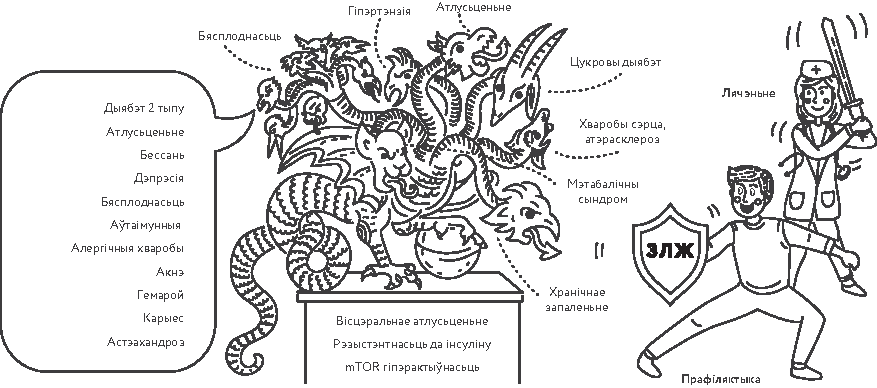
\includegraphics[width=\textwidth]{willpower/ch2/6.pdf}
\end{figure*}

Як толькі вы мяняеце лад жыцьця~--- харчаваньне, рух, сон, колькасьць стрэсу, рэжым,~--- вы бачыце паляпшэньне здароўя ў~многіх паказьніках, нават у~тых, аб якіх і не задумваліся. Зьмяняеце дыету, каб палепшыць стан скуры? Палепшыцца страваваньне, павялічыцца энэргія. Пачалі бегаць, каб схуднець? Вы станеце стрэсаўстойлівей і будзеце лепш спаць. На клеткавым узроўні гэтыя зьмены злучаныя са зьменай шэрагу сыгнальных шляхоў, галоўным зь якіх зьяўляецца бялок mTOR, які кіруе мэтабалічнай актыўнасьцю клеткі.

\subsection*{mTOR}

«Хваробы цывілізацыі» генэтычна выяўляюцца ў~выглядзе гіпэрактыўнасьці малекулярнага комплексу mTOR. Гэтае злучэньне грае ключавую ролю ў~рэгуляцыі клеткавага росту, як своеасаблівая «пэдаль газу» клеткі: з~дапамогай mTOR клетка вызначае даступнасьць калёрыяў і рэгулюе актыўнасьць мноства працэсаў. У норме mTOR мае хвалепадобную актыўнасьць, калі пэрыяды павышэньня яго актыўнасьці зьмяняюцца пэрыядамі зьніжэньня. Падчас актыўнага mTOR адбываецца сынтэз рэчываў і рост клеткі, падчас зьніжэньня актывуюцца працэсы аўтафагіі (натуральная рэгенэрацыя~--- заўв.) і аднаўленьня.

\infobox{Залішняя актыўнасьць mTOR паскарае старэньне, парушае працу імунітэту, узмацняе сыстэмнае запаленьне, скарачае працягласьць жыцьця, паскарае рост пухлінаў, павялічвае рызыку нэўрадэгенэратыўных захворваньняў.}

Нездаровае харчаваньне (пераяданьне, дробавае харчаваньне, высокая вугляводная нагрузка, лішак малака, мяса і цукру) у~спалучэньні з~гіпадынаміяй узмацняюць актыўнасьць mTOR. Некаторыя навукоўцы так і называюць «хваробы цывілізацыі»~--- mTOR-хваробы. Апроч іншага, перагрузка калёрыямі на клеткавым узроўні ўзмацняе сыстэмнае запаленьне.

У сучасным сьвеце мы актывуем mTOR пастаянна: часта ямо на працягу вялікіх прамежкаў часу, ужываем шмат ежы, што моцна падвышае актыўнасьць mTOR (багацьце мяса, цукру, малочнага, вугляводаў). Усё гэта павялічвае рызыку шматлікіх захворваньняў, ад аўтаімунных да сардэчна-сасудзістых, пухлінавых, нэўрадэгенэратыўных, паскарае старэньне. Мы быццам цісьнем на пэдаль газу занадта моцна, што зношвае наш «аўтамабіль» і неаптымальна спальвае бэнзін.

Усе стымулятары mTOR аўтаматычна павялічваюць актыўнасьць сымпатыйнай сыстэмы. Менавіта таму чалавек, які пачынае так часта есьці, першы час можа адчуць сябе «поўным сілаў», «актыўным», «зараджаным». Аднак высокая актыўнасьць сымпатыйнай сыстэмы можа ўзмацняць стрэс, падвышаць артэрыяльны ціск, павялічваць трывогу.

\textbf{Для падтрыманьня аптымальнага здароўя варта чаргаваць пэрыяды паніжанай і падвышанай актыўнасьці mTOR.} Калі мы зьніжаем актыўнасьць mTOR, нашыя клеткі пачынаюць працэс ачысткі, хуткасьць росту запавольваецца, адчувальнасьць клетак павялічваецца, арганізм можа зьнішчаць старыя і пашкоджаныя клеткі. Калі мы падвышаем актыўнасьць mTOR, то клеткі лепш аднаўляюцца, сінтэзуюць неабходныя ім бялкі. Самы просты спосаб зьменшыць актыўнасьць mTOR~--- ня есьці ў~пэўныя інтэрвалы часу. Разнавіднасьці фастынгу (інтэрвальнае галаданьне~--- \emph{заўв.}) Разгледжаныя ніжэй. Зьнізіць яго актыўнасьць можна таксама фізычнай актыўнасьцю, пры якой адбываецца выдатак калёрыяў.

Сярод «хуткіх» прадуктаў, максімальна стымулюючых mTOR, варта вылучыць бялковыя. Чым больш у~іх мэтыяніну і ВСАА амінакіслотаў (лейцын, валін, ізалейцын), тым мацнейшая актывацыя mTOR. Да гэтых прадуктаў таксама адносяцца малочныя і некаторыя расьлінныя бялкі~--- пшанічны і соевы. Вугляводы з~высокай глікемічнай нагрузкай~--- цукар~--- таксама даюць гіпэрактывацыю mTOR. Чым часьцей вы ясьце, чым шырэйшае харчовае вакно, чым больш калёрыяў вы зьядаеце, чым больш названых прадуктаў спалучаецца разам (цукар + малочка + крухмал + мяса), тым мацнейшая стымуляцыя. 

\textbf{Дадатак ВСАА, так папулярную сярод спартоўцаў, я ня раю для паўсядзённага ўжываньня.}

«Павольныя» прадукты, такія як вугляводы зь нізкай глікемічнай нагрузкай (зеляніна, гародніна, асабліва сырыя) і тлушчы маюць самы слабы ўплыў на актывацыю mTOR. Рабіце пэрыядычна «павольныя» дні, абмяжоўвайце колькасьць «хуткіх» прадуктаў, не камбінуйце іх у~адзін прыём ежы. Напрыклад, ежце мяса з~гароднінай, а~ня з~рысам, дадавайце ў~тварог ня цукар, а~зеляніну. 

\infobox{Калі больш нагрузкі, можна больш «хуткіх» прадуктаў, калі трэба адпачыць~--- больш «павольных».}

\subsection*{Інсулінарэзістэнтнасьць}

Малекулярныя парушэньні пры mTOR-гіпэрактывацыі выяўляюцца на гарманальным узроўні ў~выглядзе інсуліна- і лептынарэзістэнтнасьці. Нават бессымптомная інсулінарэзістэнтнасьць у~здаровых людзей павялічвае рызыку сьмяротнасьці. Першапачаткова інсулінарэзістэнтнасьць паўстала як прыстасавальная рэакцыя, якая дапамагае нам выжыць ва ўмовах недахопу ежы, а~таксама абараніць важныя органы ад пашкоджаньня пры лішку нутрыентаў. Інсулінарэзістэнтнасьць у~тлушчавай тканіцы і цягліцах дапамагае стварыць абарону росту арганізма, асабліва мозгу. Гэта важна для пубэртатнага росту і цяжарнасьці, таму нядзіўна, што ў~падлеткаў і цяжарных назіраецца фізыялягічная інсулінарэзістэнтнасьць. Таксама да фізыялягічнай адносіцца начная, нізкавугляводная і запаленчая інсулінарэзістэнтнасьць.

Але часьцей за ўсё інсулінарэзістэнтнасьць пры пераяданьні і гіпадынаміі шкодная для арганізма. Па меры яе разьвіцьця памяншаецца колькасьць рэцэптараў да інсуліну, што прымушае падстраўніцу (падстраўнікавую залозу) выпрацоўваць яшчэ больш інсуліну. Калі параўнаць нас і нашых бацькоў, то ў~іх у~нашыя гады быў прыкметна меншы ўзровень інсуліну ў~крыві.

\textbf{Пры пераяданьні арганізм перастае выкарыстоўваць глюкозу належным чынам, і ў~крыві запасіцца яе лішак, які можа ня толькі пераўтварацца ў~тлушч, але і пашкоджваць розныя органы-мішэні, ад мозгу да нырак. Так адаптыўны мэханізм становіцца разбуральным. Спрабуючы абараніць нас, наша цела шкодзіць нам.}

Пры лептынарэзістэнтнасьці мозг перастае атрымліваць сыгналы аб тым, што пачуцьцё голаду задаволенае, а~энэргіі ў~арганізьме~--- дастаткова. Чалавек пачынае пераядаць, і ўсё яму здаецца мала, так фармуецца заганнае кола. Чым больш мы ямо, тым больш нам хочацца есьці.

\subsection*{Айсбэрг хваробы}

«Айсбэрг хваробы» азначае наяўнасьць у~многіх людзей даклінічных формаў хваробаў, якія ігнаруюць лекары. Вельмі часта захворваньне працякае ва ўтоеным выглядзе, бязь яркіх сымптомаў. Але адсутнасьць клінічных крытэрыяў захворваньня ня робіць яго бяскрыўдным. 

Напрыклад, толькі ў~8\,\% людзей, старэйшых за 18 гадоў, ёсьць цукровы дыябэт 2 тыпу, але пры гэтым ужо ў~15\,\% людзей ёсьць парушэньні талерантнасьці да глюкозы, а~ў 25\,\%~--- прыкметна падвышаная сэкрэцыя інсуліну.

\begin{figure}[htb!]
  \centering
  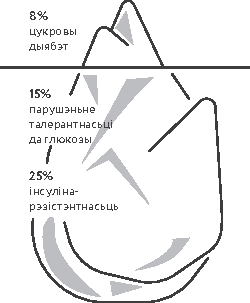
\includegraphics[scale=1.5]{willpower/ch2/7.pdf}
\end{figure}

\emph{Калі ў~чалавека з~інсулінарэзістэнтнасьцю і не разьвіваецца дыябэт, у~яго павялічваецца рызыка артэрыяльнай гіпэртэнзіі, хваробы Альцгаймэра, хваробаў сэрца, рака, памяншаецца працягласьць жыцьця. У здаровых людзей высокая інсулінарэзістэнтнасьць злучаная зь вялікімі рызыкамі для здароўя. Страшная ня тая хвароба, якая бачная, а~тая, якую мы ня бачым.}

\subsection*{Мэтабалічны сындром}

Мэтабалічны сындром аб'ядноўвае вісцэральная атлусьценьне, гіпэртанію, цукровы дыябэт і шэраг лабараторных праяваў: парушэньне ўтрыманьня тлушчаў і глюкозы ў~крыві, павышэньне ўзроўню мачавой кіслаты, павышэньне згусальнасьці крыві і да т.~п. Часта ў~лячэньні мэтабалічнага сындрому лекары спрабуюць узьдзейнічаць на такія фактары рызыкі, як высокі ўзровень трыгліцерыдаў, мачавой кіслаты, гомацыстэіну. Але барацьба з~наступствамі мэтабалічнага сындрому безь ліквідацыі базавых прычынаў неэфэктыўная.

У дасьледаваньнях зьніжэньне павышанага гомацыстэіну, высокіх трыгліцерыдаў не зьніжае рызыкі сардэчна-сасудзістых захворваньняў, зьніжэньне высокага ўзроўню мачавой кіслаты алапурынолам (блякуе ўтварэньне мачавой кіслаты) не зьніжае рызыкі пашкоджаньня нырак і разьвіцьця хранічнай нырачнай недастатковасьці і сардэчна-сасудзістых захворваньняў. Лячыць трэба чалавека, а~не аналізы!

\emph{У ЗША сыстэма аховы здароўя выдаткоўвае 75\,\% сваіх рэсурсаў на барацьбу з~наступствамі мэтабалічнага сындрому. Многія захворваньні часта суправаджаюць мэтабалічны сындром, сярод іх~--- гіпэртрафія сэрца, апноэ, сындром полікістозных яечнікаў, астэапароз, алергіі і да т.~п.}

Фізычная актыўнасьць, нізкакалярыйная дыета, інтэрвальнае галаданьне, нізкі ўзровень інсуліну, зьніжэньне IGF-1, павышэньне адчувальнасьці да інсуліну~--- усе гэтыя працэсы так ці інакш накіраваныя на зьніжэньне актыўнасьці mTOR. Некаторыя прэпараты, якія дасьледуюць як герапратэктары~--- напрыклад, рапаміцын,~--- зьяўляюцца інгібітарамі mTOR.

\subsection*{Вісцэральнае атлусьценьне}

Вісцэральнае атлусьценьне~--- аснова разьвіцьця мэтабалічнага сындрому. Гэта тлушч, які адкладаецца не ў~падскурна-тлушчавай клятчатцы, а~ў сальніку, печані, калясардэчнай сумцы, сасудах. Такі тлушч нашмат больш небясьпечны, чым падскурны, бо вылучае празапаленчыя малекулы. Вісцэральнае атлусьценьне можа сустракацца як у~худых, так і ў~поўных людзей, яго распаўсюджанасьць у~насельніцтва можа дасягаць 50\,\% і вышэй.

Пры мэтабалічным сындроме чалавек увесь час пачуваецца стомленым, зь нізкім узроўнем энэргіі і матывацыі. Сярод гарманальных парушэньняў моцна ўплываюць на самаадчуваньне павышэньне ўзроўню картызолу і норадрэналіну, у~мужчынаў~--- зьніжэньне тэстастэрону і гармону росту, у~жанчынаў~--- павышэньне тэстастэрону і андрастэндыёну. Чым шырэйшая талія ў~мужчынаў, тым ніжэйшы ўзровень тэстастэрону. Часта ў~зьніжэньні лібіда вінаваты не партнэр, а~гарманальны дысбалянс.

\infobox{Назапашваньне вісцэральнага тлушчу спрыяе свайго кшталту зьмене полу: у~мужчынаў ён зьніжае тэстастэрон, у~жанчынаў~--- павышае. Усё гэта вядзе да бясплодзьдзя, зьніжэньня лібіда, эрэктыльнай дысфункцыі.}

Чым мацнейшыя праявы мэтабалічнага сындрому, тым вышэйшая рызыка дэпрэсіі і тым цяжэй яна працякае. Яшчэ адзін сымптом~--- увесь час падвышаная трывожнасьць. Трэба трывожыцца не аб праблемах, а~аб тым, што вы пачалі занадта часта трывожыцца.

\subsection*{Пытаньні і заданьні}

1. Колькі розных праблемаў са здароўем ёсьць у~людзей, якіх вы ведаеце? Якія хваробы самыя частыя і як яны спалучаюцца адна з~адной?

2. Ці заўважалі вы, як зьніжаецца лібіда, энэргічнасьць, калі ў~чалавека зьяўляецца атлусьценьне ці іншыя захворваньні?

3. Паляпшэньне здароўя вядзе да паслабленьня ці зьнікненьня сымптомаў шматлікіх захворваньняў. Ці ведаеце вы людзей, хто, зьмяніўшы свой лад жыцьця, пазбавіўся адразу некалькіх праблемаў?


\section{Аўтаімунныя і алергічныя захворваньні}

Усё часьцей і часьцей кансультую людзей з~алергіямі і аўтаімуннымі захворваньнямі. На жаль, іх прычыну пакуль немагчыма ліквідаваць, але можна заўважна зьменшыць рызыку іх разьвіцьця ў~дзяцей. Як яны разьвіваюцца? У норме імунная сыстэма адрозьнівае «сваё» і «чужое», пры гэтым напад ідзе толькі на чужыя клеткі, а~да сваіх тканак імунітэт мае талерантнасьць. Але з~шэрагу прычынаў адбываецца збой, і імунітэт пашкоджвае свой арганізм. Цяпер 5--10\,\% насельніцтва пакутуе на аўтаімунныя і алергічныя захворваньні, у~апошнія гады хуткасьць іх распаўсюджаньня павышаецца. Гэта тыповы прыклад «хваробаў цывілізацыі»~--- яны амаль не назіраюцца ў~сучасных паляўнічых-зьбіральнікаў. Давайце разьбяромся, як дасягненьні цывілізацыі ў~выглядзе рафінаваных прадуктаў, стэрыльнасьці і антыбіётыкаў могуць выклікаць хвалю новых хваробаў.

\subsection*{Гены}

Існуе генэтычная схільнасьць да некаторых аўтаімунных захворваньняў. Імаверна, мацнейшы імунны адказ раней дапамагаў нашым продкам выжыць у~змаганьні зь небясьпечнымі інфэкцыямі, але цяпер падвышаная боегатоўнасьць імунітэту шкодзіць нам жа самім. Напрыклад, схільнасьць да расьсеянага склерозу можа быць наступствам прыстасаваньня да барацьбы з~малярыяй, а~схільнасьць да хваробы Бехцерава~--- наступствам больш эфэктыўнай абароны ад вірусаў.

\subsection*{Мікрафлёра}

Адно з~самых вывучаных плямёнаў паляўнічых-зьбі\-раль\-ні\-каў~--- племя хадза. У іх практычна няма аўтаімунных захворваньняў, затое ёсьць вельмі багатая мікрафлёра кішачніка. Магчыма, гэта зьвязана з~адсутнасьцю стэрыльнасьці, магчыма, зь іх дыетай, у~якой шмат ягадаў і караняплодаў. Да таго ж яны выкарыстоўваюць вельмі незвычайныя спосабы фэрмэнтацыі караняплодаў, каб зрабіць іх больш ядомымі~--- закопваюць у~зямлю разам з~калам жывёлаў. Гучыць ня надта апэтытна, затое ў~хадза самая разнастайная мікрафлёра ў~сьвеце, асабліва на тле вельмі беднай мікрафлёры жыхароў разьвітых краінаў.

\subsection*{Стэрыльнасьць}

Залішняя чысьціня становіцца праблемай!? Як гэта? Дасьледаваньні паказваюць, што частата алергіяў і аўтаімунных захворваньняў нашмат радзей сустракаецца ў~вёсках, у~вялікіх сем'ях, пры частым кантакце з~жывёламі. Напрыклад, чым больш у~дзіцяці братоў ці сясьцёр, тым меншая ў~яго рызыка алергічнага рыніту. З самага нараджэньня вучыцца ня толькі нашая нэрвовая сыстэма, але й імунная. Згодна з~гігіенічнай тэорыяй імунітэту~--- чым вышэйшая нагрузка на імунную сыстэму ў~раньнім дзяцінстве, тым лепей навучаецца імунітэт. І наадварот: у~«паўстэрыльным асяродзьдзі» імунная сыстэма не атрымлівае «адукацыі», што вядзе да мноства праблемаў у~дарослага чалавека. Імунітэту важная дастатковая нагрузка, якая забясьпечваецца як вонкавымі мікраарганізмамі і вірусамі, так і нашай уласнай мікрафлёрай. 

\infobox{Паступовае распаўсюджваньне мыйных, антыбактэрыйных сродкаў суправаджалася адначасовым павелічэньнем колькасьці аўтаімунных і алергічных захворваньняў.}

\begin{figure*}[htb!]
  \centering
  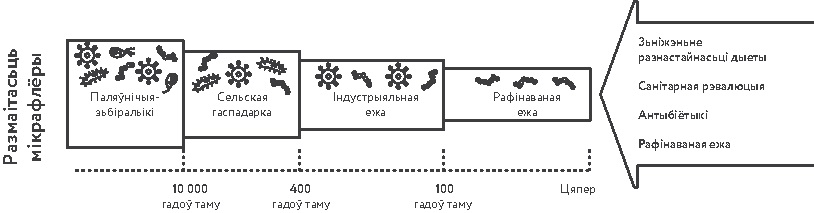
\includegraphics[width=\textwidth]{willpower/ch2/8.pdf}
\end{figure*}

\subsection*{«Новых сяброў набывай, ды старых не забывай»}

Навукоўцы прапанавалі гіпотэзу «старых сяброў»~--- яна аб тым, што для высьпяваньня імунітэту карысныя не ўсялякія вірусы, бактэрыі і паразіты, а~толькі тыя, зь якімі мы знаёмыя ўжо на працягу дзясяткаў тысячаў гадоў,то бок іх «чалавечыя» віды. Зь імі мы суіснуем у~балянсе, у~іх нізкая патагеннасьць для чалавека. Гэта, напрыклад, хелікабактэр або вастрыцы. Звыклыя зь дзяцінства гострыя рэсьпіраторныя захворваньні (ГРЗ) дапамагаюць наладзіць імунную сыстэму, а~вось новыя формы грыпу ці каранавірусу часта разбуральна ўзьдзейнічаюць на арганізм. 

Тыя, хто перахварэў на ротавірусы ў~дзяцінстве, маюць меншую рызыку захварэць на дыябэтам 1 тыпу. Пры гэтым памяншэньне колькасьці дзіцячых хваробаў у~разьвітых краінах павялічыла частату бранхіяльнай астмы на 10\,\%.

«Стэрыльны лад жыцьця» павялічвае імавернасьць хранічнага запаленьня, а~гэта ў~далейшым азначае высокую рызыку сардэчна-сасудзістых захворваньняў, дэмэнцыі, атлусьценьня. Трапляючы ў~цела, вірусы, паразіты, бактэрыі разьвіваюць супрацьзапаленчыя сеткі і павялічваюць актыўнасьць Т-рэгулятараў. Т-рэгулятары~--- гэта імунныя клеткі, якія ўмеюць стрымліваць залішнюю запаленчую рэакцыю. Такім чынам, інфэкцыі вучаць імунітэт стрымліваць сваю павышаную рэактыўнасьць.

\textbf{Вакно плястычнасьці.} Калі дзіця заразіцца вірусам Эп\-штэй\-на--Бар (вірус герпэсу~--- заўв.) у~два гады, то гэта зьніжае рызыку алергій, пасьля двух~--- ужо не. У тых, хто перахварэў на ахват да васьмі гадоў, скарачаецца імавернасьць астмы, пазьней~--- не. На працягу першых гадоў жыцьця імунная сыстэма дзіцяці праходзіць тонкую настройку, падвяргаючыся праграмаваньню пад узьдзеяньнем разнастайных антыгенаў. Вакно плястычнасьці закрываецца пасьля 5--8 гадоў. Таму бацькам важна не баяцца ўсіх бактэрыяў і вірусаў запар, а~адрозьніваць адэкватную мікробную нагрузку на прыродзе ад сапраўды небясьпечных сытуацый, накшталт знаходжаньня ў~шпіталі ці пры вялікай колькасьці людзей, у~пэрыяд успышак інфэкцыйных захворваньняў.

\textbf{Важныя разнастайнае харчаваньне сьвежай ежай, дастатковая колькасьць прэ- і прабіётыкаў, баўленьне часу на прыродзе, кантакт з~аднагодкамі, гульні на прыродзе~--- у~гразі і пяску, кантакт з~хатнімі жывёламі, мінімальнае выкарыстаньне ў~побыце антыбактэрыяльных сродкаў.}

\emph{Нават шкодныя звычкі, кшталту цягаць «казяўкі» з~носа або грызьці пазногці, зьніжаюць рызыку алергіяў. Але толькі ў~дзяцінстве~--- зьвярніце, калі ласка, увагу.}

Вядома, мы чакаем распрацоўку біяінжынэрных штамаў бактэрыяў і вірусаў, сумесь якіх зможа забясьпечыць правільнае «навучаньне» імунітэту без пабочных эфэктаў. А пакуль~--- ня будзьце, калі ласка, занадта стэрыльныя.

\subsection*{Харчаваньне}

Харчаваньне~--- гэта ня толькі вага, яно ўплывае на мноства захворваньняў. Нездаровае харчаваньне правакуе і пагаршае плынь практычна ўсіх аўтаімунных захворваньняў. Чыньнікі рызыкі могуць быць самыя розныя: гіпэрактыўнасьць mTOR, лішак солі, парушэньне мікрафлёры кішачніка, хранічнае запаленьне, дэфіцыт сонечнага сьвятла і вітаміну D, якія могуць дзейнічаць сінэргічна. Дасьледаваньні паказваюць, што сярод прадуктаў, што павялічваюць рызыку расьсеянага склерозу, знаходзіцца празьмернае спажываньне малака і мяса, небясьпечны лішак тлушчу і калёрыяў. Такі ж патэрн характэрны і для рэўматоіднага артрыту. Клятчатка, Амега-3 тлустыя кіслоты і поліфэнолы прадказальна зьніжаюць рызыку гэтых захворваньняў. 

\infobox{Шмат мяснога, малочнага, салодкага, мучнога 3--6 разоў на дзень, хай нават у~невялікіх колькасьцях, крытычна падвышае гіпэрактыўнасьць малекулярнага комплексу mTOR.}

\emph{Чым гэта небясьпечна для імуннай сыстэмы? Ёсьць Th-17 клеткі, якія стымулююць запаленчыя працэсы, а~ёсьць T-рэгулятары, якія кантралююць залішняе запаленьне,~--- пра іх мы казалі вышэй. Дык вось, навукова даведзена, што пастаянная актывацыя mTOR павялічвае выпрацоўку Th-17 і зьмяншае выпрацоўку T-рэгулятараў. Акрамя, уласна, прадуктаў, важны, вядома, і рэжым харчаваньня: калі вы ясьце позна ўвечары і ўначы, то яшчэ больш узмацняеце выпрацоўку запаленчых клетак Th-17, вытворчасьць якіх узрастае ўначы і зьмяншаецца днём.}

Добра сябе зарэкамэндавала інтэрвальнае галаданьне: фастынг зьніжае ўзровень гармону лептыну, які стымулюе размнажэньне супрацьзапаленчых Т-клетак. Але тут, як і ва ўсім, важны балянс. Калі значна зьменшыць колькасьць калёрыяў на працяглы тэрмін, то мы атрымаем прыгнёт імунітэту. Здароваму імунітэту патрэбная менавіта хвалепадобная актывацыя mTOR: пэрыядычнае ўжываньне «хуткай», mTOR-стымулёўнай ежы павінна чаргавацца з~прамежкамі «павольнай» ежы зь нізкай колькасьцю амінакіслотаў і нізкай глікемічнай нагрузкай. Менавіта такая харчовая стратэгія аптымальная для разьвіцьця Т-рэгуляраў~--- імунных клетак, якія абараняюць нас ад аўтаімунных хваробаў.

\subsection*{Соль}

Раней у~нашым жыцьці было мала солі, таму ў~арганізьме сфармаваліся сыстэмы, якія затрымліваюць натрый. 

\textbf{У сучасным сьвеце шмат таннай солі, мы сталі есьці нашмат больш натрыю і пры гэтым~--- менш калію, які маецца ў~цэльнай расьліннай ежы, яго мы ня толькі не запасім, але і выводзім лішкі пры стрэсе.}

Так соль стала адным з~чыньнікаў рызыкі атлусьценьня і мэтабалічнага сындрому, артэрыяльнай гіпэртэнзіі ды іншых захворваньняў. Больш высокая канцэнтрацыя натрыю зьяўляецца актыватарам імуннай сыстэмы, дэфіцыт ж натрыю можа аслабляць імунную сыстэму. У людзей канцэнтрацыя натрыю ў~скуры ўзрастае як адказ на пагрозу бактэрыяльнага заражэньня. Верагодна, такая рэакцыя мела эвалюцыйнае значэньне.

\emph{Пры дасьледаваньні эфэктыўнасьці імуннага адказу ў~мышэй аказалася, што «падсоленыя» макрафагі~--- клеткі, якія стравуюць і выдаляюць з~арганізма ўсё чужароднае,~--- больш актыўна зьнішчаюць бактэрыі, чым «абяссоленыя». Там, дзе ёсьць запаленьне, узровень натрыю ўзрастае.}

Высакасолевая дыета павялічвае экспрэсію празапаленчых генаў у~макрафагаў і стымулюе залішняе прадукаваньне TH17-клетак, што павышае рызыку аўтаімунных захворваньняў: лішак натрыю павышае рызыку захварэць на расьсеяны склероз, павялічвае колькасьць алергій, правакуе залішні рост бактэрыі хелікабактэр пілоры і стымулюе яе праракавы ўплыў.

\subsection*{Дэфіцыт сонечнага сьвятла}

Калі гаворка заходзіць пра аўтаімунные захворваньні, часта кажуць пра дэфіцыт вітаміну D. Сапраўды, маларухомы лад жыцьця вядзе да дэфіцыту сонечнага сьвятла, і гэты дэфіцыт павялічвае рызыку іх узьнікненьня. Невыпадкова большасьць аўтаімунных захворваньняў, напрыклад расьсеяны склероз, упершыню выяўляюцца менавіта ўзімку. 

\infobox{Існуе правіла 1000 гадзінаў: для здароўя на працягу году трэба быць на вуліцы каля трох гадзінаў на дзень.}

Гэта можа быць складана, калі вы не жывяце ў~прыватным доме альбо вулічнае асяродзьдзе агрэсіўнае і небясьпечнае. Аднак ёсьць да чаго імкнуцца. Падрабязна пра карысьць сонца і абарону ад яго~--- у~разьдзеле «Карыснае асяродзьдзе».

\subsection*{Пытаньні і заданьні}

1. Ці шмат часу вы праводзілі ў~дзяцінстве на вуліцы, зь дзецьмі, з~жывёламі, на прыродзе? А як бавяць час вашыя дзеці?

2. Ці часта вы выкарыстоўваеце антыбіётыкі і ці заўсёды гэта абгрунтавана?

3. Колькі хвілінаў на дзень вы бываеце на сонцы?


\section{Хранічнае запаленьне}

Запаленьне~--- гэта комплексны адказ арганізма на пашкоджаньне, выкліканае рознымі чыньнікамі, ад траўмы да інфэкцыі. Вынікам гэтай рэакцыі становіцца ліквідацыя пашкоджаньня і аднаўленьне арганізма, што ідзе нам на карысьць. Аднак часта імунны адказ зацягваецца, тады гаворка ідзе пра хранічнае запаленьне. Хранічнае запаленьне наносіць сур'ёзную шкоду арганізму і павялічвае рызыку заўчаснага старэньня, раку, дыябэту, нэўрадэгенэратыўных захворваньняў ды іншых паталёгіяў.

\emph{Свой узровень запаленьня можна ацаніць па лабараторных тэстах, напрыклад здаўшы аналізы на такія маркеры, як С-рэактыўны бялок або ІЛ-6.}

Калі моцная траўма ці інфэкцыя дае гострае запаленьне, якое, як полымя, загараецца і хутка згасае, то хранічнае запаленьне~--- гэта тленьне вугольля. У сучасным ладзе жыцьця зьявілася шмат прычынаў хранічнага запаленьня. Узмацняе запаленьне нездаровае харчаваньне (ежа позна ўвечары, высокаглікемічныя вугляводы, перапрацаваная ежа, смажанае, вэнджанае, таксіны і да т.~п.), недасып, недахоп або залішняя фізычная актыўнасьць, нізкая разнастайнасьць мікрафлёры, шкоднае асяродзьдзе (бруднае паветра, шум г.~д.), стрэс, адзінота і адсутнасьць падтрымкі.

\emph{\textbf{Узровень С-рэактыўнага бялку} ў~паляўнічых-зьбіральнікаў ніжэйшы, чым у~жыхароў разьвітых краінаў. Дасьледаваньні на Філіпінах і ў~Эквадоры паказваюць, што ўзровень С-рэактыўнага бялку прыкметна ніжэйшы, а~ўзровень супрацьзапаленчага ІЛ-10 вышэйшы, чым у~заходніх краінах, незалежна ад ІМЦ.}

Чым меншая антыгенная нагрузка ў~дзяцінстве, тым вышэйшы ўзровень СРБ у~дарослых. Праблема сучаснага стэрыльнага сьвету заключаецца ў~тым, што зьніжэньне колькасьці вонкавых інфэкцыяў і зьніжэньне ўнутранай разнастайнасьці мікрафлёры вядзе да ўзмацненьня празапаленчай рэакцыі. Уплываць на ўзровень запаленьня могуць самыя розныя аспэкты жыцьця, ад хранічных інфэкцыяў да псыхалягічнага стрэсу. Запаленьне ня толькі паскарае старэньне, але й павялічвае рызыку мноства захворваньняў як на лякальным узроўні (напрыклад, гастрыт, выкліканы хелікабактэрам у~страўніку, павялічвае рызыку раку страўніка), так і на сыстэмным узроўні (рызыка сардэчна-сасудзістых захворваньняў, нэўрадэгенэратыўных і псыхічных захворваньняў), закранае самыя розныя сыстэмы органаў, напрыклад можа выклікаць анэмію пры нармальным спажываньні жалеза.

У людзей як істот сацыяльных стрэс таксама зьвязаны з~актывацыяй імуннай сыстэмы. Таму чым меншы ўзровень сацыяльнай падтрымкі, тым вышэйшыя маркеры запаленьня. Больш высокі ўзровень сацыяльнай падтрымкі зьмяншае ўзровень запаленьня і рызыкі ня толькі дэпрэсіі, але й астмы, сардэчна-сасудзістых захворваньняў і інш. Некантраляваны стрэс павялічвае ўзровень ІЛ-6, і чым вышэйшы яго ўзровень, тым мацнейшая рызыка выгараньня.

\subsection*{Стрэс}

Хранічны стрэс прыводзіць да актывізацыі стрэсавай вэгетатыўнай сыстэмы (сымпатаадрэналавай) і зьніжэньню працы антыстрэсавай (парасымпатыйнай) сыстэмы. Галоўным нэрвам парасымпатыйнай сыстэмы зьяўляецца вагус (блукальны нэрв), сярод функцый якога~--- кантроль сыстэмнага запаленьня. Высокі тонус вагусу важны для зьніжэньня запаленьня. Стымуляцыя вагусу і парасымпатыйнай сыстэмы зьніжае рызыку многіх захворваньняў, ад хваробы Паркінсана да дэпрэсіі і аўтаімунных хваробаў. Прэпараты, якія стымулююць парасымпатыйную сыстэму або блякуюць сымпатыйную, зьніжаюць выкід празапаленчых цытакінаў. 

\emph{Розныя спосабы актывацыі вагусу разгледжаныя ў~разьдзеле «Стрэсаўстойлівасьць».}

\textbf{Хранічнае запаленьне} зьвязанае з~павелічэньнем у~крыві празапаленчых малекулаў, у~тым ліку С-рэактыўнага бялку, ІЛ-6, ФНП, TNF, фібрынагену і шэрагу іншых маркераў. Запаленьне перабудоўвае працу клетак, выкарыстоўваючы празапаленчы рэгулятарны шлях NF-kB. Хранічнае запаленьне, як іржа, праймае наша цела і падточвае здароўе. Ёсьць меркаваньне, што павелічэньне запаленьня шчыльна зьвязанае з~працэсам старэньня (inflammaging). Больш актыўныя запаленчыя гены, больш высокія запаленчыя маркеры скарачаюць працягласьць жыцьця, а~супрацьзапаленчыя рэчывы~--- павялічваюць. Клеткі арганізма, якія старэюць і перастаюць дзяліцца, могуць пачаць выпрацоўваць шмат празапаленчых малекулаў. Навукоўцы распрацоўваюць спосабы іх ліквідацыі або перапраграмаваньня.

\textbf{Харчаваньне і атлусьценьне.} Узмацняе запаленьне і рознае клеткавае «сьмецьце», клеткавыя і малекулярныя пашкоджаньні ў~тканках у~выніку, напрыклад, глікацыі (калі падвышаны ўзровень глюкозы ў~крыві прымушае яе незваротна зьвязвацца з~нашымі клеткамі) або ўтварэньня сшывак. Чым больш пашкоджаньняў, тым мацней мяняецца імунагеннасьць нашых тканак, што выклікае запаленчую рэакцыю арганізма. Папулярным робіцца бодыпазітыў у~дачыненьні да лішняй вагі, калі людзі намаўляюць сябе, што гэта нармальна. Але ж лішні тлушч~--- гэта крыніца хранічнага запаленьня, і чалавек як быццам гарыць. Яго хочуць выратаваць, а~ён кажа, што гэта не небясьпечна.

\infobox{Прадукты харчаваньня могуць валодаць як празапаленчымі, так і супрацьзапаленчымі ўласьцівасьцямі. Напрыклад, у~ягадах і гародніне шмат прыродных саліцылатаў, якія зьніжаюць запаленьне гэтак жа, як зьніжаюць запаленьне і асьпірын, і аліўкавы алей першага адціску. А вось рафінаваныя вугляводы, перапрацаванае мяса, цукар узмацняюць запаленьне.}

Эфэкты нездаровага харчаваньня ўзмацняюць запаленьне праз пашкоджаньне мітахондрыяў у~клетках. Запаленьне пагаршае здароўе і праз цэнтральныя мэханізмы, напрыклад пашкоджваючы працу гіпаталямуса і гіпакампа, што яшчэ мацней паскарае старэньне. Таксама запаленьне зьніжае адчувальнасьць да інсуліну і парушае мэтабалізм, вядзе да зьніжэньня ўзроўню дафаміну.

Хранічнае запаленьне прыводзіць да ўзмацненьня паступленьня таксінаў, празапаленчых цытакінаў і клетак імуннай сыстэмы ў~мозг. Там яны могуць выклікаць другасныя пашкоджаньні, якія ўзмацняюць нэўразапаленьне. Чым вышэйшы ўзровень у~крыві С-рэактыўнага бялку і ІЛ-6, тым горш для гематаэнцэфалічнага бар'еру (мяжа паміж мозгам і крывёй). Павышаны ўзровень запаленьня здольны пашкоджваць розныя тканкі, напрыклад аслабляць рост цяглічнай масы і павышаць рызыку саркапэніі.

Таму нядзіўна, што ступень цяжкасьці дэпрэсіі і біпалярнага разладу карэлююць з~узроўнем С-рэактыўнага бялку ў~крыві. Зьніжэньне хранічнага запаленьня дабратворнае для мозгу. Ведаць узровень запаленьня важна, бо гэта гаворыць і пра іншыя рызыкі. Напрыклад, павышаны халестэрын пры павышаным СРБ нашмат небясьпечнейшы, чым яго больш высокі ўзровень, але пры нармальным СРБ. Для зьніжэньня запаленьня важна саніраваць усе магчымыя агмені хранічнай інфэкцыі: інфэкцыі зубоў і ротавай поласьці, вушныя інфэкцыі, мочапалавыя, гастрыты і да т.~п.

\textbf{Бар'еры.} Адна з~умоваў здаровага функцыянаваньня арганізма~--- гэта падтрыманьне вонкавых і ўнутраных бар'ераў. Чым менш бар'ераў, тым мацнейшымі могуць быць парушэньні нашага здароўя і хутчэйшым старэньне. І тут значэньне маюць ня толькі ўнутраныя бар'еры, але і стан скуры! Па меры сталеньня чалавека скура становіцца больш сухой і менш трывалай. А гэта вядзе да ўтварэньня мікратрэшчынаў і пашкоджаньняў. На пашкоджаньні арганізм адказвае звыкла~--- празапаленчай рэакцыяй і павелічэньнем сінтэзу празапаленчых цытакінаў. А паколькі плошча скуры досыць вялікая, дык гэта аказвае сыстэмны эфэкт.

\emph{У дасьледаваньні (зь невялікай выбаркай) вывучаўся ўплыў элемэнтарнага ўвільгатненьня скуры за ўсё цела ў~пажылых звычайным крэмам двойчы на дзень. Высьветлася, што за гэты час узровень інтэрлейкін-1 бэта, інтэрлейкін-6 і фактар нэкрозу пухліны альфа зьнізіліся, прычым узровень інтэрлейкіну-1 бэта і інтэрлейкіну-6 зьнізіўся да ўзроўню трыццацігадовых.}

Пазьбягайце пашкоджаньня вашых унутраных бар'ераў. Для абароны кішачніка нармалізуйце харчаваньне і мікрафлёру, для гематаэнцэфалічнага бар'еру пазьбягайце траўмаў галавы, вісцэральнага атлусьценьня, хранічных інфэкцыяў і запаленьня, недасыпу, стрэсу і гіпадынаміі. Сачыце за станам скуры, пазьбягайце фотастарэньня, пашкоджаньняў, насіце самае камфортнае і зручнае адзеньне і абутак, каб нідзе ня муляла, сачыце за скурай ступняў.

\emph{Многія рэчывы, якія ёсьць у~жывёльнай і расьліннай ежы, валодаюць супрацьзапаленчым эфэктам (каратыноіды, амэга-3, поліфэнолы і інш.), рыхтык як і многія лекавыя прэпараты (асьпірын, мэтфармін, статыны і інш.).}

\subsection*{Запаленьне і зубы} 

Карыес~--- гэта адна з~«хваробаў цывілізацыі», зьвязаная з~залішнім спажываньнем мяккай і вугляводнай ежы. Карыес зьяўляецца ў~чалавечай гісторыі толькі пры пераходзе на сельскую гаспадарку. Рызыка карыесу павышаецца пры зьніжэньні самаачышчэньня ротавай поласьці з~прычыны нізкай выпрацоўкі сьліны, «жавальнай ленасьці», выкарыстаньня прадуктаў з~загушчальнікамі, напрыклад ксантану, гуаравай камедзі. Беларускі назоў глютэну~--- «клейкавіна», і ён, акрамя ўсяго іншага, можа «прыклейваць» часьцінкі крухмалу да зубоў, што затрымліваюцца ў~ротавай поласьці і зьяўляюцца пажыўным асяродзьдзем для разьвіцьця патагеннай мікрафлёры. 

\infobox{Назапашваючыся ў~міжзубных прамежках, дзяснавай баразёнцы, прышыевай вобласьці зубоў і ў~іншых месцах, мяккая ежа спрыяе прагрэсаваньню карыесу. Пастаянныя перакусы таксама зьніжаюць эфэктыўнасьць самаачышчэньня ротавай поласьці.}

Важна штодня чысьціць зубы, абавязкова выкарыстоўваць нітку і чысьціць язык (можна адмысловай шчоткай або кавалачкам марлі), а~таксама паласкаць рот вадой пасьля кожнага прыёму ежы. Ня варта выкарыстоўваць паласкальнікі для рота, бо яны шкодзяць звычайнай мікрафлёры ротавай поласьці. А вось аральныя прабіётыкі, якія ўтрымліваюць карысныя штамы, напрыклад S. Salivarius BLIS K12, могуць ня толькі зьнізіць рызыку карыесу, але й пазбавіць ад непрыемнага паху з~рота. Дбайнае жаваньне цьвёрдай ежы, якое патрабуе багатага сьлінавыдзяленьня, паляпшае кровазабесьпячэньне органаў ротавай поласьці, спрыяе лепшаму ачышчэньню і дапамагае гарманічнаму разьвіцьцю шкілета твару ў~дзяцей.

Калі ў~вас было пратэзаваньне зубоў, выдаленьне, то ў~выніку гэтага маглі ўтварыцца каналы, якія могуць зьяўляцца крыніцай запаленьня. Важна зрабіць трохмерную тамаграфію сківіц, каб выключыць запаленьне. Выкарыстоўвайце сучасныя спосабы пратэзаваньня, каб пазьбегнуць крыніц запаленьня.

\subsection*{Пытаньні і заданьні}

1. Які ў~вас узровень запаленьня?

2. Ці ёсьць у~вас хранічныя інфэкцыі (зубы, прастата) або аутоімунные захворваньні?

3. Ці шмат вы ясьце перапрацаванай ежы?


\section{Атлусьценьне}

Многія людзі, калі прыходзяць працаваць са мной, пачынаюць з~пахуданьня. Сапраўды, падтрыманьне нармальнай вагі~--- гэта адначасова і самая эфэктыўная прафіляктычная мера, і самая складаная багата для каго. Фармальная парада «проста меней еж» не працуе для большасьці. Доўгі час навукоўцы спрабуюць знайсьці прычыны атлусьценьня, і іх колькасьць такая, што просты агляд заняў бы ўсю гэтую кнігу. Таму я хачу расказаць пра \textbf{дзьве гіпотэзы атлусьценьня~--- эвалюцыйную і сацыяльна-псыхалягічную}. Яны не выключаюць адна адну, а, хутчэй, дапаўняюць.

Імаверна, атлусьценьне~--- гэта парушаны адаптыўны адказ арганізма зьмененыя ўмовы навакольнага асяродзьдзя. Мэханізмы захаваньня калёрыяў, якія дапамагалі выжываць у~старажытнасьці, сёньня шкодзяць нам.

\subsection*{Эвалюцыйная гіпотэза атлусьценьня}

Паводле гэтай тэорыі за атлусьценьне адказны комплекс генаў, якія забясьпечваюць падтрыманьне і назапашваньне энэргіі пры дэфіцыце харчаваньня.

Пры ладзе жыцьця паляўнічых-зьбі\-раль\-ні\-каў даступнасьць ежы часта вар'іравалася. Сэзоны багацьця зьмяняліся голадам~--- так званы цыкль голад--баляваньне. Таму замацоўвалася здольнасьць арганізма назапашваць лішкі ежы і спальваць іх на тле павышэньня актыўнасьці і голаду. 

\infobox{Не было лядоўняў, гатовых прадуктаў, службаў дастаўкі, а~здабываць ежу атрымлівалася не заўсёды. Вось і выяўляецца, што нашы продкі заўжды практыкавалі пэрыядычнае галаданьне і не перакусвалі абы-чым.
Цяпер мы сутыкнуліся з~сытуацыяй, калі ежа даступная пастаянна, але гэтыя мэханізмы па-ранейшаму прымушаюць нас адкладаць «на чорны дзень». Калі раней ва ўмовах дэфіцыту ежы яе лішак дапамагаў нам выжыць, дык цяпер ва ўмовах багатае празьмернасьці нам дапамагае ўмеранасьць.}

З усіх відаў ежы найбольшую каштоўнасьць для выжываньня ўяўляюць прадукты з~высокай удзельнай калярыйнай шчыльнасьцю. Калі раней многія караняплоды і садавіна былі даступныя сэзонна, а~здабыць мёд або буйную жывёлу ўдавалася не заўсёды, арганізм заахвочваў такія знаходкі выкідам дафаміну, і чалавек імкнуўся зьядаць ежу цалкам, у~карысьць.

\emph{Вугляводы ў~выглядзе брокалі не выклікаюць асаблівага апэтыту, а~вось у~выглядзе эклера~--- зусім іншая справа. Чым вышэйшая шчыльнасьць калёрыяў і глікемічны індэкс, чым больш тлушчу і бялку, тым мацнейшы наш апэтыт і вышэйшая рызыка пераяданьня.}

Мы таксама схільныя пераядаць салёнае (дэфіцыт солі ў~прыродзе) і смажанае ці вэнджанае (даступнасьць калёрыяў з~тэрмічна апрацаванай ежы вышэйшая)~--- і ўсе гэтыя прадукты правакуюць жаданьне зьесьці іх у~запас.

\emph{17 мільёнаў гадоў таму ў~пэрыяд чарговага пахаладаньня ў~нашых вельмі далёкіх продкаў адбылася мутацыя ў~гене ўрыказы, які рэгулюе абмен мачавой кіслаты. У выніку гэтага ўзровень мачавой кіслаты ў~крыві вырас. Мачавая кіслата~--- прадукт раскладаньня фруктозы, такім чынам, калі мы ямо шмат фруктозы, гэта зьніжае адчувальнасьць да інсуліну, што павялічвае колькасьць тлушчу. Значыць, мы больш эфэктыўна ператвараем цукар у~тлушч. Болей тлушчу~--- вышэйшая імавернасьць выжыць у~неспрыяльны пэрыяд. Акрамя гэтага, фруктоза зьніжае адчувальнасьць да гармону сытасьці лептыну, што правакуе пераяданьне.} \textbf{Для нас гэта шкодна, але для выжываньня карысна, бо сэзон сасьпелай садавіны кароткі, і трэба зьесьці яе зь лішкам, каб назапасіць дастаткова тлушчу.}

Падобная гісторыя адбылася з~алькаголем. Мы навучыліся яго засвойваць не ад добрага жыцьця, а~ад неабходнасьці, каб выжыць, есьці нават тую садавіну, якая ўпала і забрадзіла. 10 мільёнаў гадоў таму ў~агульнага продка чалавека і вышэйшых малпаў адбылася мутацыя ў~гене алькагольдэгідрагеназе, што ў~40 разоў павялічыла хуткасьць расшчапленьня этанолу. Дзякуючы гэтаму нашы продкі былі ў~стане ня толькі зьесьці забрадзілую садавіну, але й вярнуцца назад на дрэва. Цукар і алькаголь увогуле маюць надзіва шмат агульнага. Па-першае, у~прыродзе мы атрымлівалі іх з~аднаго прадукту~--- садавіны, сасьпелай і забрадзілай. Па-другое, цукар і алькаголь выклікаюць аднолькавыя праблемы ў~печані і правакуюць інсулінарэзістэнтнасьць. Па-трэцяе, залежнасьць ад алькаголю і салодкага зьвязаная з~адным і тым жа аддзелам галаўнога мозгу. Ну і нарэшце, цукар і алькаголь аднолькава зьніжаюць сілу волі, вядуць да дэпрэсіі і выгараньня.

\textbf{Рафініраваньне і перапрацоўка прадуктаў} заўважна ўплываюць на тое, як яны дзейнічаюць на наш арганізм. Напрыклад, яблык і яблычны сок узьдзейнічаюць па-рознаму. Сок, здробнены і без харчовых валокнаў, хутка праходзіць праз страўнік як вадкасьць ды інтэнсіўна ўсмоктваецца, выклікаючы моцны гарманальны водгук і пікавую канцэнтрацыю цукру. Цьвёрды яблык затрымліваецца ў~страўніку, стравуецца плыўна, клятчатка запавольвае ўсмоктваньне цукру, і засваеньне праходзіць мякчэй і карысьней. \textbf{Сок шкодзіць, а~суцэльны фрукт~--- не.}

Значэньне мае і тып вугляводаў. Цяпер людзі ядуць шмат мучнога і крупаў. Такія канцэнтраваныя вугляводы з~высокай глікемічнай нагрузкай рэзка павялічваюць узровень глюкозы, выклікаюць запаленчую рэакцыю ў~кішачніку. Частае і залішняе ўжываньне ў~ежу такіх вугляводаў зьмяншае адчувальнасьць да інсуліну, што павялічвае рызыку запаленьня, дэпрэсіі, дыябэту. \emph{Найбольш высокае ўжываньне такіх вугляводаў павялічвае рызыку сьмерці на 30\,\% пры параўнаньні з~найболей нізкім.}

А вось вугляводы з~караняплодаў і гародніны станоўча ўплываюць на здароўе. Таму рэч ня ў~грамах вугляводаў у~вашай дыеце, а~ў пэўных прадуктах, зь якіх вы гэтыя вугляводы атрымліваеце.

Падобная сытуацыя і з~тлушчамі: адбылося павелічэньне спажываньня транстлушчоў, якія павялічваюць рызыку сардэчна-сасудзістых захворваньняў. У нашым рацыёне зьявілася прыкметна больш Амэга-6 тлустых кіслот, якія ўтрымліваюцца ў~танных алеях накшталт сланечнікавага, соевага, кукурузнага і могуць аказваць празапаленчае ўзьдзеяньне, перадусім ва ўмовах дэфіцыту Амэга-3. 

\emph{Утрыманьне лінолевай кіслаты (Амэга-6) у~падскурным тлушчы павялічылася зь 9.1\,\% у~1959 годзе да 21.5\,\% у~2008-м, г.~зн. вырасла на 136\,\%. Атрымліваецца, што ў~целе ў~нас два лішнія кіляграмы лінолевай кіслаты. Мы~--- тое, што мы ямо.}

\subsection*{Эканомныя гены}

Пры галаданьні ці стрэсавых рэакцыях уключаюцца мэханізмы захаваньня энэргіі, калі цела зьмяншае актыўнасьць і спажываньне энэргіі ў~тых сыстэмах органаў, якія не зьяўляюцца неабходнымі для выжываньня. Можна зэканоміць на працы цягліцаў і шчытавіцы (шчытападобнай залозы), на імуннай і рэпрадуктыўнай сыстэмах і г.~д.

\infobox{Рэжым дэфіцыту~--- гэта комплексныя зьмены арганізма, ад нежаданьня рухацца, зьніжэньня настрою і матывацыі да цягі да высокакалярыйнай ежы і адключэньня пачуцьця насычэньня.}

Нашу схільнасьць набіраць вагу~--- і меней рухацца пры гэтым~--- разглядаюць як «зімовую сьпячку». Так, рэзістэнтнасьць да лептыну і інсуліну, павышэньне ўзроўню свабодных тлустых кіслотаў дапамагае эвалюцыйна эканоміць энэргію пры неспрыяльных умовах. Але ў~сучасных умовах ахоўная рэакцыя становіцца паталягічнай. Мы як мядзьведзі: увесь час ямо, назапашваем тлушч, чакаем зіму, пачуваемся санлівымі, але так і не ўпадаем у~сьпячку.

\emph{Эпігенэтычныя тэорыі атлусьценьня апісваюць мноства цікавых «рашэньняў» арганізма, пачынаючы з~моманту зачацьця. Актыўнасьць шэрагу генаў, якія ўдзельнічаюць у~энэргетычным абмене, можа зьмяніцца пад узьдзеяньнем розных чыньнікаў, напрыклад голаду ці стрэсу, і схільнасьць да атлусьценьня будзе закладзеная яшчэ ўнутрывутробна, пачаўшы перадавацца ў~спадчыну ў~межах некалькіх пакаленьняў.}

\subsection*{Гіпэрфагія (пераяданьне)}

З вынаходствам лямпачкі мы сталі вячэраць пазьней і багацей. Адыліж ежа, якую мы ямо ў~розны час дня, па-рознаму ўплывае на здароўе. Позьняя ежа павялічвае рызыкі для здароўя, лішак сьвятлодыёднага выпраменьваньня з~высокай доляй сьвятла сіняга спэктру ад розных прыладаў зьбівае нашы ўнутраныя гадзіньнікі й загастрае пачуцьцё голаду. Гэта \textbf{цыркадная гіпэрфагія}~--- пераяданьне празь зьбітыя біярытмы.

\emph{Мы нават i не ўспрымаем колькасьці святла ўвечар і ўначы як фактар, што ўплывае на пераяданьне. Тым часам, рызыка атлусьценьня павялічваецца на 33\,\%, калі чалавек спіць з улучаным сьвятлом.}

А вось і \textbf{геданістычная гіпэрфагія}: мы пераядаем, каб атрымаць больш задавальненьня. Калі ў~людзей зьніжаецца задавальненьне ад жыцьця, то ежа~--- самы танны і даступны спосаб сябе «парадаваць». Мацней за ўсё паднімаюць узровень аднаго з~«гармонаў шчасьця» дафаміну прадукты з~вялікай колькасьцю вугляводаў, цукру, тлушчу, смажанага і салёнага, а~таксама іх камбінацыі.

\textbf{Стрэсавая гіпэрфагія}~--- гэта калі людзі ядуць не для задавальненьня фізычнага голаду, а~для вырашэньня эмацыйных праблемаў: супакоіцца, заесьці, падняць настрой, заглушыць нуду. Хранічны стрэс павялічвае ўзровень гармону голаду грэліну і выклікае пераяданьне: узровень зьедзеных калёрыяў неўзаметку павялічваецца, здольнасьць кантраляваць свой апэтыт і голад некуды зьнікае.

Стрэсу цяпер стала больш, за 15 хвілінаў прагляду навінаў чалавек можа ўбачыць фота і відэа такой колькасьці трагедыяў, катастрофаў і забойстваў, якую іншы чалавек у~Сярэднявеччы ня ўведаў бы і за дзесяць гадоў.

Калі раней ежа была рытуалам, то сучасны чалавек можа паесьці дзе заўгодна: на хаду, у~машыне, за працоўным сталом, у~кінатэатры, у~ложку. Разбурэньне культуры харчаваньня прыводзіць да таго, што мы лянуемся старанна жаваць і праглынаем ежу кавалкамі, ямо хутка і неўсьвядомлена, гледзячы ў~тэлефон або тэлевізар, усё радзей сядзім за адным сталом, аддаючы перавагу «перахапленьню чаго-небудзь» на самоце. Павелічэньне хуткасьці паглынаньня ежы, ежа ў~стрэсе значна павялічваюць колькасьць зьедзеных калёрыяў і памяншаюць задавальненьне ад працэсу. Як правіла, у~такіх умовах людзі часьцей выбіраюць гатовую ежу, якая вылучаецца нізкай біялягічнай каштоўнасьцю і высокай калярыйнасьцю.

\subsection*{Даступнасьць ежы}

Калі раней пры адсутнасьці лядоўняў і гатовых прадуктаў людзі елі радзей і не перакусвалі, то цяпер вакол нас на адлегласьці выцягнутай рукі мноства відаў ежы, мы можам замовіць анляйн што заўгодна~--- і гэтае нешта прыедзе да нас на працягу паўгадзіны. Пачынаючы з~50-х гадоў у~людзей паступова расла колькасьць прыёмаў ежы. Прадуктаў становіцца больш, але разнастайнасьць нашага харчаваньня зьніжаецца. Нашы продкі ўжывалі дзясяткі відаў жывёлаў і расьлінаў, розныя травы, ягады, грыбы, птушак, елі шмат фэрмэнтаванай ежы. Цяпер жа мы ямо абмежаваны набор прадуктаў: ялавічына, сьвініна, курыца, соя, пшаніца, кукуруза, малочка і да т.~п. складаюць большасьць калёрыяў у~шмат каго.

\subsection*{Сацыяльна-псыхалягічная гіпотэза атлусьценьня (гіпотэза харчовай няўпэўненасьці)}

Устаноўлена: чым ніжэйшыя даходы, тым вышэйшая няўпэўненасьць у~заўтрашнім дні і тым вышэйшая частасьць атлусьценьня. Гэтая заканамернасьць працуе толькі ў~разьвітых краінах, дзе нават бедныя пласты насельніцтва могуць дазволіць сабе купляць шмат калярыйнай ежы. Харчовая няўпэўненасьць~--- гэта агульнае абазначэньне магчымых у~будучыні праблемаў з~доступам да ежы. Для нашага мозгу, як мы памятаем, вельмі важнае пытаньне выжываньня. А пытаньне выжываньня вырашаецца ў~будучыні.

Чым вышэйшы у~нас узровень рэсурсаў сёньня, чым вышэйшая упэўненасьць у~заўтрашнім дні, чым больш разьвітая здольнасьць плянаваць, тым вышэйшая «харчовая ўпэўненасьць». Гэтая сувязь выявілася і ў~іншых дасьледаваньнях, прычым яе сталі называць «парадоксам беднасьці-атлусьценьня», калі пры недахопе грошай або нерэгулярным заробку назіралася павелічэньне частасьці атлусьценьня.

\textbf{Харчовая няўпэўненасьць}~--- гэта абмежаваньні або немагчымасьць атрымліваць паўнавартасную ежу сацыяльна прымальнымі спосабамі. Харчовая няўпэўненасьць не зьвязаная з~аб'ектыўным дэфіцытам, яна можа выяўляцца ў~выглядзе боязі за будучыню, няўпэўненасьці ў~заўтрашнім дні, зьніжэньнем прыстасоўвальных магчымасьцяў. Сыгналы харчовай няўпэўненасьці~--- гэта павышэньне ўзроўню стрэсу, зьвязанага са звужэньнем гарызонту плянаваньня. 

\infobox{Працяглы хранічны стрэс прыгнятае прэфрантальную кару, якая адказвае за плянаваньне. Гэта вядзе да таго, што чалавек пачынае «жыць адным днём», што, па сутнасьці, і зьяўляецца харчовай няўпэўненасьцю.}

Мозг вырашае праблему даступным спосабам~--- наборам вагі: тлушчавыя дэпо арганізма ў~такім выпадку працуюць як важны мэханізм выжываньня. Але захоўваньне тлушчу ў~іх таксама мае свой кошт для арганізма~--- ад павышэньня рызыкі шэрагу захворваньняў да зьніжэньня рухальнай актыўнасьці. 

Нават намёк на цяжкія часы і праблемы заўважна ўзмацняе пераяданьне. Зрэшты, гэтая стратэгія працавала толькі ў~старажытнасьці, калі нам пагражаў голад. Сёньня ж нам нібы зразумела, што піца ня вырашыць нашы працоўныя, фінансавыя, асабістыя праблемы, але ўсё роўна падкорка дзейнічае па-старому.

\emph{У дасьледаваньні прапаноўвалі на выбар два гатункі цукерак: першыя былі адзначаныя як нізкакалярыйныя, другія~--- высокакалярыйныя. За сьпінамі дасьледнікаў вісеў плякат, дзе ў~адным выпадку былі нэўтральныя словы і сказы, а~ў іншым~--- тыя, што выклікаюць стрэс і трывогу: барацьба, недахоп, няшчасьце, выжываньне і інш. Там, дзе быў стрэс, удзельнікі зьядалі больш высокакалярыйных цукерак. Іншыя дасьледнікі вывучалі колькасьць калёрыяў, зьедзеных спартовымі фанатамі падчас посьпехаў іх каманды. Пры паразах колькасьць ужытых высокакалярыйных прадуктаў прыкметна павялічвалася.}

Больш высокі сацыяльны статут зьвязаны з~больш эфэктыўным абменам рэчываў: дамінантныя жывёлы маюць больш высокі энэргетычны выдатак, чым недамінантныя. Да таго ж ніжэйшы сацыяльны статус і ніжэйшае становішча ў~гіерархіі зьвязаныя з~залішнім спажываньнем калёрыяў.

Незалежна ад тыпу дыеты і пажыўнасьці ежы, людзі і жывёлы зь ніжэйшым сацыяльным статусам у~дасьледаваньнях ядуць нашмат больш калёрыяў, чым астатнія. У чалавека ўзровень адукацыі, даходу, стрэсу заўсёды зьвязаны з~энэргетычнай, гэта значыць калярыйнай шчыльнасьцю харчаваньня. Павышэньне сацыяльнага стрэсу вядзе да павелічэньня спажываньня ежы і хуткага набору вагі. Таму чым вы прыгажэйшыя і здаравейшыя, тым меней вам хочацца есьці. А чым вы таўсьцейшыя, тым горш сябе адчуваеце, ад стрэсу яшчэ больш ясьце, замыкаючы заганнае кола.

\subsection*{Пытаньні і заданьні}

1. Як у~вас зьвязаны стрэс і пераяданьне? Як зьмяняецца ваш стыль харчаваньня ва ўмовах моцнага, гострага і хранічнага стрэсаў?

2. Ці ўплывае на ваш рацыён нявызначанасьць у~будучыні, цьмяныя пэрспэктывы, ваша самаацэнка?

3. Якія прадукты прымушаюць вас больш за ўсё пераядаць? Ці трымаеце вы іх у~сябе дома?


\section{Дэпрэсія}

Дасьледаваньні сярод плямёнаў паляў\-ні\-чых-зьбіральнікаў, якія літаральна перасьледуюць нас на працягу ўсяго разьдзел, паказалі, што ў~гэтых «дзяцей прыроды» альбо адсутнічае дэпрэсія і яе эквіваленты, альбо назіраюцца адзінкавыя выпадкі. Пры гэтым у~«цывілізаваных» краінах дэпрэсія назіралася ўжо з~антычных часоў. 

\infobox{Мэлянхолія, іпахондрыя, сплін~--- чым актыўнейшым было жыцьцё, тым часьцей у~людзей выяўляліся станы рознай ступені прыгнечанасьці.}

Цяпер дэпрэсія~--- адно зь вядучых захворваньняў. Кожны чацьвёрты амэрыканец пакутуе ад клінічнай дэпрэсіі на працягу жыцьця, а~ў 2030 годзе гэта будзе вядучая прычына непрацаздольнасьці. Гэта глябальная эпідэмія і галоўная прычына, зь якой штогод зьдзяйсьняюць самагубства больш за мільён чалавек ва ўсім сьвеце. Прычыны дэпрэсіі могуць як унутранымі, так і вонкавымі: дэпрэсіі бываюць мэтабалічнымі і стрэсавымі, могуць быць зьвязаныя з~захворваньнямі (напрыклад, гіпатэрыёз) або вонкавымі фактарамі (напрыклад, дэфіцыт сонца). Сардэчна-сасудзістыя захворваньні або атлусьценьне могуць прыводзіць да разьвіцьця дэпрэсіі, і наадварот, дэпрэсія павялічвае рызыку сардэчна-сасудзістых захворваньняў і атлусьценьня. Мэханізмы ўзьнікненьня дэпрэсіі тлумачыць мноства тэорый~--- ад кагнітыўнай да монаамінавай, якая гаворыць пра дысбалянс сэратаніну, норадрэналіну, дафаміну.

\emph{Дэпрэсія магла ўзьнікнуць як пабочны эфэкт эвалюцыі імуннай сыстэмы, карысны для выжываньня. Падчас дэпрэсіі нашы паводзіны зьмяняюцца: дрымотнасьць, апатыя, мінімум руху~--- усё гэта зьніжае і расход калёрыяў. Зьніжэньне актыўнасьці пры інфэкцыйных захворваньнях магло зьнізіць колькасьць кантактаў паміж індывідамі і, адпаведна, запаволіць распаўсюджваньне хваробы. Нават парушэньні сну пры дэпрэсіі могуць быць зьвязаныя з~павелічэньнем часу няспаньня для выратаваньня ад драпежнікаў.}

\subsection*{Запаленьне і дэпрэсія}

Даўно была заўважаная сувязь паміж дэпрэсіяй і запаленчай рэакцыяй. У людзей з~дэпрэсіяй больш «раздражняльны» імунітэт і вышэйшыя маркеры запаленьня нават у~пэрыяд рэмісіі. Тыя 20--30\,\% людзей з~дэпрэсіяй, якія застаюцца неадчувальнымі да антыдэпрэсантаў, маюць найболей высокія паказьнікі запаленчых маркераў. Запаленьне ўзмацняе трывогу: дасьледаваньні паказваюць, што ўзроўні празапаленчых цытакінаў ІЛ-1 і ІЛ-6 прыкметна вышэйшыя ў~крыві і мозгу людзей, якія пакончылі з~сабой. Запаленьне ў~мозгу ўплывае на актыўнасьць працы нэўрамэдыятарных сыстэмаў (сэратанін, дафамін, глутамат), а~таксама прыгнятае актыўнасьць працы дафамінавай сыстэмы. 

Усе супрацьзапаленчыя прэпараты і дадаткі ў~цэлым зьніжаюць і рызыку дэпрэсіі.

\subsection*{Стрэс і дэпрэсія}

Больш высокі ўзровень сацыяльнай падтрымкі, кантроль запаленчых маркераў і іх карэкцыя могуць палепшыць наш мэнтальны стан пры дэпрэсіі, трывозе, выгараньні, а~таксама зьнізіць рызыку ня толькі дэпрэсіі, але й астмы, сардэчна-сасудзістых захворваньняў і інш.

\emph{Як трапна заўважыў Карл Юнг, «сталасьць чалавека вызначаецца тым, як шмат нявызначанасьці ён можа вытрымаць».}

Сёньня наш сьвет называюць VUCA-сьвет: volatility (нестабільнасьць), uncertainty (нявызначанасьць), complexity (складанасьць) і ambiguity (неадназначнасьць) і нам патрабуецца больш псыхалягічнай устойлівасьці, каб даць яму рады. Мы можам сфармуляваць свой VUCA-адказ: Vision (бачаньне сваіх каштоўнасьцяў), Understanding (разуменьне таго, што адбываецца), Clarity (яснасьць успрыманьня), Agility (гнуткасьць і адаптыўнасьць). Замест супраціўленьня зьменам нам важна навучыцца супрацьстаяць інфармацыйнаму шуму, перапрацоўваць шмат інфармацыі, кіраваць сваёй энэргіяй і станам, адаптавацца і вучыцца на працягу ўсяго жыцьця. Бо супраціў, некантраляванасьць, непрадказальнасьць~--- усё гэта фактары рызыкі выгараньня і дэпрэсіі.

\subsection*{Паводзіны і дэпрэсія}

Пры дэпрэсіі мы пачынаем мысьліць іначай, нашмат дакладней ацэньваем рызыкі і пагрозы. 

\infobox{Тэорыя зьніжэньня нявыгаднай паводзіннай актыўнасьці мяркуе, што нашы адмоўныя эмоцыі дапамагаюць у~далейшым пазьбягаць няслушных рашэньняў.}

Пры дэпрэсіі мозг мацней факусуецца на праблемах, увесь час іх пракручвае, і, тэарэтычна, гэта можа дапамагчы нам вырашыць глябальныя жыцьцёвыя выклікі. Але не, гэта не рэкляма дэпрэсіўных станаў: зьніжэньне энэргіі і матывацыі ў~адказ на неэфэктыўныя дзеяньні магло першапачаткова дапамагаць, але ў~наш час зьяўляецца дэзадаптыўным.

Як і на любыя іншыя «хваробы цывілізацыі», на дэпрэсію дабратворна ўплывае практычна кожны з~рэсурсаў здароўя, якія мы будзем разьбіраць у~наступных разьдзелах: харчаваньне, сон, рухальная актыўнасьць, стрэсаўстойлівасьць, сацыяльнае асяродзьдзе, навакольнае асяродзьдзе ды іншыя фактары. Лёгкія і сярэднія формы дэпрэсій рацыянальна пачаць лячыць акурат са зьмены ладу жыцьця. Шчыра ацаніце свой стан~--- і наперад.

\subsection*{Хранічныя болі і саматаформныя разлады}

Ад гэтай праблемы мне галава баліць! Паводле ацэнак, да 30\,\% людзей пакутуюць ад розных хранічных болевых сындромаў, а~да 20\,\% людзей на прыёме ў~лекара маюць саматаформныя разлады, г.~зн. болевыя сындромы без канкрэтнае арганічнае нагоды. Прычына такіх боляў~--- не ў~парушэньнях у~тым месцы, дзе баліць, а~ў галаве. Псыхагенны боль зьвязаны з~парушэньнямі апрацоўкі інфармацыі і часта з~дэфіцытам нэўрамэдыятараў, напрыклад дафаміну, што прыпадабняе яго да дэпрэсіі. Але для такога дыягназу трэба цалкам выключыць арганічныя прычыны болю.

Хранічныя болі часта спадарожнічаюць хваробам, часта бываюць самастойным сымптомам, маскай дэпрэсіі, могуць выяўляцца ў~выглядзе фібраміялгіі, хранічнай тазавай болі, хранічнай паясьнічнай болі, болі ў~грудзях, цяжкасьцямі ўдыху, пачуцьцём камяка ў~горле, сындромам раздражнёнага кішачніка і да т.~п. Многія зь людзей зьведваюць непатрэбнае і часта небясьпечнае лячэньне. Напрыклад, пры сындроме раздражнёнага кішачніка, як і пры дэпрэсіі, эфэктыўныя кагнітыўна-паводзінная тэрапія і антыдэпрэсанты.

\subsection*{Пытаньні і заданьні}

1. Ці былі ў~вас эпізоды клінічнай дэпрэсіі? Ці ёсьць людзі з~дэпрэсіяй сярод вашых сваякоў і знаёмых?

2. Ці адчуваеце вы часам віну, ці схільныя да самакрытыкі, ці бываюць у~вас думкі пра сьмерць? Як часта ўзьнікаюць такія думкі і ці надоўга затрымліваюцца?

3. Ці часта ў~вас бывае прыгнечаны настрой, страта задавальненьня ад жыцьця, працяглая стомленасьць, парушэньне здольнасьці канцэнтравацца і колькі па часе доўжацца гэтыя сымптомы?


\section{Блізарукасьць}

Блізарукасьць~--- гэта клясычная хвароба цывілізацыі. Так, у~канадскіх эскімосаў яе практычна не было, а~20--25\,\% іх дзяцей ужо блізарукія. Насуперак міфам, дасьледаваньні не знаходзяць прамой сувязі паміж напругай вачэй пры чытаньні і блізарукасьцю. \textbf{Праблема аказалася ў~іншым~--- у~колькасьці часу, які дзеці праводзяць на вуліцы.}

\emph{Старажытнарымскі медык Гален, які жыў у~II стагодзьдзі нашай эры, зьвязваў разьвіцьцё блізарукасьці з~малой колькасьцю сонечных промняў, якія трапляюць у~вока. У Сэуле, дзе школьнікі праводзяць на вуліцы менш за гадзіну, блізарукасьць дасягае 95\,\% (!), а~ў Аўстраліі, дзе дзеці гуляюць больш за тры гадзіны на дзень, блізарукія каля 30\,\%.}

Такім чынам, усё проста: чым больш дзіця праводзіць часу ў~двары, тым меншая рызыка блізарукасьці. Тлумачачы гэты фэномэн, адны навукоўцы прыпісвалі ахоўны эфэкт агульнаму ўзроўню асьветленасьці (10.000 люкс на вуліцы і максімум 500 у~класе), або фізычнай актыўнасьці, або спэктральным асаблівасьцям сонечнага сьвятла. У канчатковым выніку мелі рацыю апошнія. Рэч у~тым, што ў~сьвятлодыёдным сьвятле практычна цалкам адсутнічаюць хвалі 290--420 нм, а~для актывацыі ахоўнага дзеяньня дафаміну ў~сеткавіцы патрэбныя хвалі менавіта гэтага спэктру.

Пакуль лекары прапануюць у~дапамогу «акулярыкам» нейкія зарадкі або адмысловы пальмінг (тэхніка паслабленьня вачэй У. Бэйтса~--- заўв.), сапраўдныя мэханізмы ўзьнікненьня блізарукасьці па-навуковаму прыўкрасныя: гэтае сонца і дафамін. Так, у~сеткавіцы ёсьць свае дафамінавыя нэўроны, і чым вышэйшы ўзровень дафаміну, тым меншая рызыка блізарукасьці. Дафамін зьяўляецца тым чыньнікам, які прыгальмоўвае фібрабласты і спыняе залішні рост вочнага яблыка. 

\emph{Навукоўцы нават вывелі мышэй з~паніжаным дафамінам у~сеткавіцы, у~якіх разьвівалася міяпія без усялякага напружанага чытаньня.}

\textbf{Дык што ж рабіць?} У экспэрыментах 40-хвілінная актыўнасьць па-за школай прывяла да зьніжэньня колькасьці хворых на блізарукасьць на 25\,\% на працягу трох гадоў. Гульні на сьвежым паветры ня менш за тры гадзіны ў~дзень~--- гэта найлепшы навуковы спосаб прафіляктыкі блізарукасьці і запаволеньня яе разьвіцьця. 

\emph{«Міяпія перастане прагрэсаваць, калі вы адправіцеся ў~марское падарожжа»,~--- пісаў у~пачатку XX стагодзьдзя брытанскі афтальмоляг Генры Эдвард Джулер.}

\textbf{Што ж, разумная парада. Болей сонца і дафаміну!}

У мяне блізарукасьць пачала разьвівацца ў~школе, я доўгі час насіў акуляры. Але яны мне не падабаліся, бо абмяжоўвалі поле зроку. Пасьля 30 гадоў я зрабіў апэрацыю па лазернай карэкцыі зроку, і адзінае, аб чым шкадую, што не зрабіў гэтага раней. Паўнавартасны зрок дае магчымасьць успрымаць навакольны сьвет больш дакладна, больш яскрава. Гэта павялічвае энэргічнасьць і актыўнасьць, бо візуальнае ўспрыманьне~--- гэта ежа для мозгу.

Між іншым, аслабленьне сэнсарных стымулаў вядзе да дэпрэсіі і павялічвае рызыку нэўрадэгенэратыўных захворваньняў. Навукоўцы выявілі, што апэрацыя па ўхіленьні катаракты зьніжае рызыку дэпрэсіі і хваробы Альцгаймэра. Устаноўка слыхавога апарата валодае такім жа эфэктам. Мне шкада людзей, якія лічаць, што трэба зьмірыцца з~узроставым зьніжэньнем зроку і слыху і ніяк не карэктаваць іх. 

\textbf{У любым узросьце важна карміць свой мозг якаснай «ежай», якая «здабываецца» з~дапамогай добрага зроку і слыху, рэгулярнага руху і разнастайных прыемных узьдзеяньняў на цела. І я буду рэгулярна нагадваць вам пра гэта.}

\textbf{Корміце мозг.} Важна падтрымліваць у~добрым стане і іншыя органы пачуцьцяў. Аслабленьне нюху з~узростам~--- часты сымптом раньніх стадый нэўрадэгенэратыўных захворваньняў, іх яшчэ можна эфэктыўна спыніць на гэтым этапе. Пагаршэньне нюху падвойвае рызыку дэменцыі ў~бліжэйшыя 5 гадоў. А вось у~пацыентаў у~коме аднаўленьне нюху~--- гэта добрая прагнастычная прыкмета. Можна палепшыць нюх: трэнаваць яго, лячыць рынасінусіты; ёсьць і шэраг экспэрымэнтальных спосабаў, ад інтраназальнага інсуліну да ствалавых клетак. Трэніроўка нюху ня толькі паляпшае здольнасьць адрозьніваць пахі, але й стымулюе глябальныя працэсы нэўраплястычнасьці. Дасьледаваньні паказваюць, што трэніроўка нюху паляпшае вэрбальныя здольнасьці мацней, чым, скажам, рашэньне судоку.

\subsection*{Пытаньні і заданьні}

1. Якая ў~вас гастрыня зроку? Як вы яе кампэнсуеце (акуляры, лінзы, карэкцыя)? Ці добры ў~вас слых? Смак?

2. Ці адчуваеце вы стомленасьць вачэй? Як часта?

3. Ці ёсьць у~вас магчымасьць глядзець удалячынь на працягу дня? Гэта карысна для раслабленьня цягліцаў вока.


\section{Акнэ і аксэлерацыя}

За школьным часам у~мяне былі жудасныя высыпаньні на твары. Змагаліся зь імі рознымі спосабамі: прыпякалі, выціскалі, але ніхто так і не прапанаваў мне заняцца харчаваньнем. Толькі паступіўшы ва ўнівэрсытэт, я вывучыў гэтае пытаньне, зьмяніў лад жыцьця і пазбавіўся ад праблемы. Тэма гэтая настолькі актуальная, што відэа «Чым вы корміце акнэ?» на маім Youtube-канале сабрала максімальную колькасьць праглядаў у~параўнаньні зь іншымі відэа. \textbf{Гэта нядзіўна, бо з~кожным годам ад акнэ пакутуе ўсё больш і больш дарослых людзей.}

Многія лічаць акнэ лякальнай часовай касмэтычнай праблемай, але насамрэч гэта вонкавая праява «хваробаў цывілізацыі». Акнэ не сустракаецца ў~паляўнічых-зьбіральнікаў: дасьледчыкі плямёнаў у~Парагваі і ў~Папуа-Новая Гвінэя не сустрэлі ніводнага выпадку акнэ сярод падлеткаў або дарослых.

\emph{Дасьледнікі падрабязна апісалі зьяўленьне і распаўсюджваньне акнэ ў~інуітаў (эскімосаў Паўночнай Амэрыкі) па меры іх пераходу на заходні стыль харчаваньня. Прычым гэтае распаўсюджваньне нарастае: калі раней акнэ сустракалася пераважна ў~падлеткаў (да 85\,\%), дык цяпер яно сустракаецца ў~15--40\,\% дарослых. Больш за тое, існуе ўстойлівая тэндэнцыя да павышэньня распаўсюджваньня «дарослага акнэ».}

Сярод прычынаў узьнікненьня акнэ~--- спалучэньне генэтыкі і ладу жыцьця. \textbf{Як і ў~іншых «хваробаў цывілізацыі», у~аснове акнэ ляжыць mTOR-гіпэрактывацыя:} лішак росту эпітэліяльных клетак, фалікулярны гіпэркератоз (закаркаваньне вусьцяў валасяных фалікулаў), павышаная сэкрэцыя клусных залоз (сэбарэя), запаленьне (як агульнае, так і лякальнае), парушэньне скурнай мікрафлёры (Propionibacterium acne і яе дысбалянс зь іншымі ахоўнымі скурнымі штамамі).

Ключавым мэханізмам запуску зьяўляецца гарманальны, андрагенавы дысбалянс на лакальным узроўні. Як правіла, у~аналізах пры акнэ лішак андрагенаў выяўляецца рэдка. Касмэтычныя падыходы да лячэньня акнэ працуюць, але глыбінныя прычыны застаюцца. Таму важны сыстэмны падыход, які забясьпечыць добрую фізычную форму, сон, нізкі ўзровень стрэсу, адсутнасьць запаленчых працэсаў, добрую адчувальнасьць да інсуліну і да т.~п. Напрыклад, дыета зь нізкім глікемічным індэксам на 50\,\% зьніжае выяўленасьць акнэ за тры месяцы. Для дасягненьня мэтабалічных паляпшэньняў патрабуецца час і праца над сабой.

Паляпшэньне сыстэмнага здароўя дапаможа вам ня толькі выглядаць лепш, але й зьменшыць рызыку шэрагу захворваньняў. Даведзена, што акнэ зьяўляецца маркерам шэрагу іншых хваробаў, сярод якіх астма, ангіна, сінусіт, харчовая алергія, рэфлюкс-эзафагіт. А тыя дарослыя, у~якіх акнэ выяўлялася ў~юным узросьце, у~будучыні маюць вышэйшую рызыку эндамэтрыёзу, раку грудзей, падкарэньніцы (падкарэннай залозы), мэляномы і інш.

\subsection*{Харчаваньне і аксэлерацыя}

Вельмі важна кантраляваць харчаваньне і лад жыцьця падлеткаў, але нават ад прытомных бацькоў часта можна пачуць меркаваньне, што «дзіця само лепш ведае, што есьці», «яму малако, булкі і цукар патрэбныя для росту», «усё роўна, што дзіця есьць, пакуль вага нармальная~--- усё добра». Насамрэч абмежаваньне пэўных прадуктаў у~рацыёне для дзіцяці яшчэ важнейшае, чым для дарослага, бо дзяцінства закладвае траекторыю здароўя на ўсё жыцьцё. Залішняе харчаваньне дзяцей выяўляецца ў~выглядзе аксэлерацыі~--- паскарэньня росту і больш раньняга палавога пасьпяваньня. Высокі рост дзяцей радуе бацькоў, але радасьць гэтая заўчасная. 

\infobox{Адваротны бок аксэлерацыі~--- гэта амаладжэньне захворваньняў, у~першую чаргу хваробаў старэньня.}

Цяпер мы бачым тэндэнцыю «амаладжэньня» многіх відаў раку, інсультаў, нэўрадэгенэратыўных захворваньняў. Сёньня навукоўцы падлічваюць «распаўсюджваньне хваравітасьці», а~менавіта колькасьць гадоў, страчаных па стане здароўя, і колькасьць сьмерцяў, зьвязаных з~хранічнымі захворваньнямі. 

\emph{З 1990 па 2010 год працягласьць хранічных захворваньняў узрасла: для дыябэту на 30\,\%, для хваробы Альцгаймэра на 17\,\%. За апошнія 30 гадоў мінулага стагодзьдзя ў~Брытаніі падвоілася колькасьць выпадкаў раку грудзей.}

Існуе пэўная логіка ў~разьвіцьці: чым раней узьнікаюць парушэньні, тым хутчэй яны прагрэсуюць. Таму амаладжэньне інсультаў, інфарктаў і атлусьценьня цалкам заканамернае: паглядзіце на дзяцей 2--3 гадоў, якія спажываюць фастфуд і цукар. 

Ад першапачатковых парушэньняў да праблемаў з~сэрцам праходзіць ад 10 да 25 гадоў. Праз 10--20 гадоў пасьля пачатку мэтабалічнага сындрому разьвіваецца і прагрэсуе атэрасклероз, у~далейшым магчымыя яго ўскладненьні~--- інфаркт і інсульт. Сярод хворых з~мэтабалічным сындромам сьмяротнасьць ад ішэмічнай хваробы сэрца ў~23 разы вышэй, чым у~сярэднім у~насельніцтва.

Часта можна ўбачыць, як бацькі купляюць розныя прысмакі дзецям і абавязкова «ўсім пароўну». Але ці сапраўды гэта ўсім пароўну? У пэдыятрыі, каб правільна разьлічыць дазоўку прэпарата, выкарыстоўваюць паказьнік дозы на кіляграм масы цела. Калі мы возьмем сярэдняе марозіва ў~70 грамаў, чатырохгадовае дзіця вагой 14 кг і яго бацьку вагой 80 кг, то дзіця атрымлівае марозіва ў~дазоўцы 5 грамаў на кіляграм масы цела, а~бацька~--- усяго толькі 0,87 грама на кіляграм масы цела, што ў~5,7 разоў менш. Ці зможаце вы зьесьці за раз амаль 6 плямбіраў і як будзеце пасьля гэтага сябе адчуваць? 

\infobox{Такім чынам, спажываючы прысмакі ў~роўнай колькасьці з~дарослымі, дзіця атрымлівае калярыйна-цукровы ўдар амаль у~5--6 разоў мацнейшы.}

\textbf{Можна прадоўжыць прычынна-выніковыя сувязі.}

Чым больш жанчына набірае вагу падчас цяжарнасьці, тым вышэйшая вага дзіцяці. 

Чым больш дзіця спажывае сумесяў (у адрозьненьне ад груднога гадаваньня), тым хутчэй яно расьце. 

Чым хутчэй узрастае вага, тым раней уключаецца рэпрадуктыўны цыкль. 

Праз скарачэньне тэрміну разьвіцьця арганізма, паводле ўнівэрсальнага біялягічнага закону, скарачаецца і працягласьць жыцьця чалавека.

Чым раней уключаецца палавы цыкл, тым мацней расьце рызыка дыябэту, атэрасклерозу, гарманальна-залежных ракаў і нэўрадэгенэратыўных захворваньняў.

У прыватнасьці, акнэ~--- гэта тыповая прыкмета аксэлерацыі.

\textbf{Важна:} нельга дапускаць лішак хутка засваяльнай ежы з~моманту цяжарнасьці і далей па меры росту дзіцяці. Хутка засваяльная ежа~--- гэта стымулятар mTOR. Найбольшую небясьпеку ўяўляюць малочныя прадукты (гаворка не пра грудное малако, вядома), затым ідуць жывёльныя бялкі, цукры, сокі і ўсе прадукты з~высокай глікемічнай нагрузкай. І асабліва варта пазьбягаць салодкіх малочных прадуктаў~--- ёгурту, сыркоў або тартоў. Калі дзіця ўвесь час сілкуецца сокамі, сушкамі ды іншымі харчовымі заменьнікамі, гэта павялічвае ўдар у~разы. \textbf{Няхай вашыя дзеці ядуць нармальную здаровую ежу, нават калі вы хочаце іх парадаваць або лічыце, што ўсё можна, пакуль яны растуць.}

\subsection*{Пытаньні і заданьні}

1. У вас было (ці ёсьць цяпер) акнэ? Што правакуе яго зьяўленьне?

2. Ці была ў~вас залішняя маса цела ў~дзяцінстве? Ці часта вы пераядалі?

3. Ці займаліся вы ў~дзяцінстве спортам?


\section{Лад жыцьця, лібіда і фэртыльнасьць}

«Мужчыны цяпер ня тыя», -- уздыхаюць жанчыны. І сапраўды, у~разьвітых краінах у~мужчынскага насельніцтва падае ўзровень тэстастэрону. Трэнд гэты пачаўся ў~1920--1930-х. Апошнія 50 гадоў узровень тэстастэрону ў~крыві мужчынаў падае на 1\,\% у~год: у~канцы 80-х у~65-гадовага мужчыны было на 17\,\% тэстастэрону больш, чым у~яго аднагодка ў~2004 годзе. Зьмяняюцца і суадносіны гармонаў~--- для сучаснага чалавека характэрны больш высокі ўзровень эстрагену, прагестэрону і тэстастэрону. Таксама назіраецца прыкметнае зьніжэньне лібіда і фэртыльнасьці ў~абодвух палоў: людзі менш займаюцца сэксам, радзей бяруць шлюб. Колькасьць народкаў памяншаецца на 1,5\,\% у~год у~мужчынаў у~ЗША і на 3\,\% у~год у~мужчынаў у~Эўропе і Аўстраліі.

\emph{Арганізм жанчыны прыстасаваны да таго, каб нараджаць вялікую колькасьць дзяцей і доўга іх гадаваць. Павелічэньне колькасьці мэнструальных цыкляў у~сучасных жанчынаў можа быць зьвязана з~падвышанай рызыкай раку.}

Зьмена гарманальнага балянсу тэс\-тас\-тэ\-рон--эстраген уплывае ня толькі на тое, як выглядаюць жанчыны, але й на тое, як гавораць. Так, за апошнія 50 гадоў мы бачым у~жанчынаў значнае зьніжэньне вышыні голасу~--- з~229 Гц да 206 Гц. Адныя дасьледнікі лічаць, што прычынай зьяўляецца непасрэдна пераразьмеркаваньне ўплыву і ўлады, бо на ўзровень тэстастэрону ўплывае статус і дамінаваньне.

Каля 25\,\% параў, якія маюць праблемы з~фэртыльнасьцю, атрымліваюць дыягназ «бясплоднасьць нявызначанага генэзу». Ёсьць меркаваньне, што сама меней траціна ўсіх выпадкаў бясплодзьдзя~--- наступства хранічнага стрэсу і дэпрэсіі, прычым ужываньне антыдэпрэсантаў таксама зьяўляецца чыньнікам бясплодзьдзя. А яшчэ вялікі ўклад у~праблему ўносяць і парушэньні харчаваньня.

\emph{У адным з~дасьледаваньняў было выяўлена, што ў~тых, хто ня можа зацяжарыць, самыя высокія маркеры стрэсу (альфа-амілаза). Верхнія ўзроўні гэтага маркера павялічваюць рызыку бясплодзьдзя ў~сярэднім у~два разы. Іншыя дасьледаваньні пацьвердзілі гэтыя назіраньні і адзначылі неабходнасьць выкарыстаньня тэхнікаў рэляксацыі для павелічэньня фэртыльнасьці.}

\infobox{Варта заўважыць, што менавіта мужчынская дэпрэсія мацней за ўсё ўплывае на фэртыльнасьць пары: у~60\,\% выпадкаў бясплодзьдзе сустракалася ў~параў, дзе ў~дэпрэсіі быў мужчына. Такая заканамернасьць не выяўлялася ў~выпадку дэпрэсіі ў~жанчынаў.}

Стрэс нэгатыўна ўзьдзейнічае і на якасьць спэрмы. 

Кантроль і зьніжэньне ўзроўню стрэсу напрамую ўплывае на ўзроўні ФСГ і ЛГ, эстрагену і тэстастэрону. \textbf{Выснова: вучыцеся кіраваць сваімі рэакцыямі і зьніжаць узровень хранічнага стрэсу.}

Акрамя псыхалягічнага ціску, да крыніцаў хранічнага стрэсу адносяцца начны шум, сьветлавое забруджваньне ды іншыя раздражняльныя фактары навакольнага асяродзьдзя. Напрыклад, зьмены сьветлавога рэжыму могуць адмоўна ўплываць на фэртыльнасьць. 

\emph{У млекакормячых мэлятанін павялічвае фэртыльнасьць.}

\subsection*{Харчаваньне}

Зьмена харчаваньня таксама аказвае выразнае ўзьдзеяньне на палавыя гармоны. У мужчынаў вісцэральнае атлусьценьне вядзе да зьніжэньня ўзроўню тэстастэрону, эрэкцыі, лібіда. Нават проста лішняя маса цела без атлусьценьня ўжо дакладна павялічвае частасьць бясплодзьдзя.

У дасьледаваньнях нармалізацыя харчаваньня і ўмеранае пахуданьне павысілі лібіда нават у~стройных здаровых мужчынаў. Існуе здагадка, што інсулінарэзістэнтнасьць у~мужчынаў са звычайнай масай цела можа памяншаць фэртыльнасьць. Чым большая талія, тым меней тэстастэрону ў~мужчыны.

\textbf{Вісцэральнае атлусьценьне ў~мужчынаў зьніжае ўзровень тэстастэрону, а~ў жанчынаў~--- павялічвае яго, і гэта, падобна, адна з~прычын зьмяненьняў у~карціне сьвету.}

У жанчынаў павышаны ўзровень інсуліну прыводзіць да падвышанай выпрацоўкі андрагенаў у~яечніках. А гіпэрандрагенія можа прыкметна зьнізіць фэртыльнасьць. Больш за тое, высокі ўзровень тэстастэрону падчас цяжарнасьці моцна ўзьдзейнічае на мозг плода, напрыклад уплывае на гендэрныя перавагі або ступень адоранасьці, а~таксама павялічвае рызыку ўзьнікненьня аўтызму.

\subsection*{Пытаньні і заданьні}

1. Ацаніце сваё лібіда. Як на яго ўплываюць зьмены ў~вашым ладзе жыцьця: адпачынак, стрэс, недасып, харчаваньне?

2. Як часта вы займаецеся сэксам? Гэта больш ці менш, чым вам хочацца?

3. Якая ў~вас вышыня голасу? Паспрабуйце гаварыць крыху вышэй і крыху ніжэй. Як гэта ўзьдзейнічае на навакольных?


\section{Даўгалецьце і старэньне}

Вельмі часта я чую фразу: «У старажытнасьці жылі на прыродзе, елі арганічную ежу, але ў~35 гадоў паміралі». Таксама шырока распаўсюджанае ўяўленьне, што працягласьць нашага жыцьця радыкальна павялічылася. Насамрэч гэта ня так. Працягласьць нашага жыцьця павялічылася нязначна, проста рэзка зьнізілася сьмяротнасьць, а~гэта зусім розныя рэчы. Больш людзей пачалі дажываць да старасьці, але нашмат даўжэй людзі жыць не пачалі. Давайце разьбяромся, чаму ўзьнік гэты міт «сярэдняй тэмпэратуры па шпіталі» і як ён узьнік.

\emph{Хоць многія перакананыя ў~тым, што ў~антычнасьці людзі жылі да 35 гадоў, яшчэ ў~7 стагодзьдзі да н.э. Гесіёд пераконваў мужчынаў не жаніцца да 30 гадоў з~прычыны негатоўнасьці. Рымляне падзялялі гэтае меркаваньне: у~палітыку можна было пайсьці толькі пасьля 30 гадоў, а~стаць консулам рымлянін мог адно пасьля 40. У старажытнагрэцкіх законах было прапісана, што на вайну бралі ўсіх мужчынаў да 60 гадоў, а~вось стаць суддзёй маглі людзі толькі старэйшыя за 60.}

Згодна з~дасьледаваньнямі архэоляга Крысьцін Кейв, у~традыцыйным грамадстве 600--700 гадоў н.э. (пры адсутнасьці сучаснага ўзроўню разьвіцьця мэдыцыны) людзі даволі часта паміралі ва ўзросьце 70 гадоў.

\textbf{Разгледзім чатыры аспэкты гэтага скажэньня. Прычына першая~--- памылкі вызначэньня.}

\textbf{Другая прычына~--- вельмі высокі ўзровень гвалту.} Мы жывем у~самы мірны час. Сьмяротнасьць сярод паляўнічых-зьбіральнікаў большая на 15--60\,\% з~прычыны міжпляменных канфліктаў. Калі б так ваявалі ў~XX стагодзьдзі, то страты ў~дзьвюх сусьветных войнах склалі б больш за 2 мільярды чалавек. 

\textbf{Трэцюю прычыну~--- дзіцячую звышсьмяротнасьць}~--- вы можаце самі прасачыць у~мэтрычных кнігах нават XIX стагодзьдзя, яна была вельмі высокая і таму моцна зьмяншала чаканую працягласьць жыцьця. 

\textbf{Чацьвёртая прычына~--- інфэкцыйныя захворваньні}, эпідэміі, сьмяротнасьць пры родах ды іншыя мэдыцынскія прычыны сьмерці, якія цяпер кантралююцца нашмат лепш.

Як толькі праходзілі небясьпечныя дзіцячыя гады, імаверная працягласьць жыцьця, напрыклад у~віктарыянскую эпоху, была падобная сучаснай. Так, дзяўчынка ва ўзросьце пяці гадоў мела чаканую працягласьць жыцьця 73 гады, а~хлопчык~--- 75 гадоў. Нават калі мы возьмем сучасныя дзікія плямёны паляўнічых-зьбіральнікаў, то імавернасьць дажыць да 15 гадоў складае 55\,\%, але ўжо пасьля 15 чаканая працягласьць жыцьця складае 58 гадоў. А калі паляўнічыя-зьбіральнікі пераадольваюць мяжу ў~45 гадоў (не памерлі пры родах, не забітыя ў~канфліктах), то жывуць яшчэ 29 гадоў~--- да 65--67.

\emph{Працягласьць жыцьця ў~наш час вырасла перадусім дзякуючы паляпшэньню харчаваньня, якаснай вадзе, гігіене, кантролю інфэкцыйных захворваньняў (антыбіётыкі, вакцынацыя, санітарыя і да т.~п.), транспартнай бясьпецы, выкарыстаньню некаторых прэпаратаў (антыгіпэртэнзіўныя і да т.~п.).}

\textbf{Хоць сярэдняя працягласьць жыцьця расьце, максімальная, мабыць, дасягнула мяжы і не мяняецца з~1980-х гадоў. У сярэднім шанцы дажыць да 100 гадоў у~нас павышаюцца, але 120 гадоў~--- гэта біялягічная мяжа даўгалецьця, і колькасьць супэрдоўгажыхароў апошнім часам не асабліва павялічылася.}

Навукоўцы зьвярнулі ўвагу, што па меры ўзмацненьня жорсткасьці ўліку ўзросту колькасьць супэрдоўгажыхароў зьніжаецца. Імаверна, іх шаноўны ўзрост часта~--- вынік маніпуляцыяў або памылак ацэнкі. Цяпер мы ня бачым новых рэкордаў даўгалецьця, ня бачым павелічэньня сярэдняга ўзросту сярод доўгажыхароў, не назіраем зьніжэньня сьмяротнасьці сярод тых, хто перасягнуў 11-гадовую мяжу, да якой высокая рызыка дзіцячых інфэкцыяў. Гэта ўсё паказвае на тое, што шанцы павялічыць працягласьць жыцьця 120+ без радыкальных прарываў і тэхналёгіяў мізэрныя. Магчыма, гэта зьвязана з~тым, што наша даўгалецьце мае пэўныя біялягічныя абмежаваньні. Некаторыя навукоўцы лічаць, што нашы мэханізмы старэньня і так ужо аптымізаваныя, што чалавек~--- доўгажывучы від, таму тыя ўмяшаньні, якія працуюць на мухах і мышах, для чалавека не эфэктыўныя. Такім чынам, абсалютная большасьць існых падыходаў у~мэдыцыне хутчэй зьніжаюць рызыку заўчаснае сьмерці, а~не падаўжаюць жыцьцё, і накіраваныя на прафіляктыку, запаволеньне і лячэньне хваробаў.

\subsection*{Старэньне як хвароба хваробаў}

Згаданыя хваробы цывілізацыі маюць паміж сабой шмат агульнага. Усе яны бяруць пачатак у~мэханізмах старэньня і самі паскараюць старэньне. Пакуль навукоўцы спрачаюцца, ці лічыць старэньне хваробай, несумненна, мэханізмы, якія прыводзяць да сардэчна-сасудзістых захворваньняў, дыябэту, пухлінаў, нэўрадэгенэратыўных захворваньняў, астэапарозу, катаракты, артрытаў і старэньня, маюць шмат агульнага.

\emph{Атлусьценьне паскарае старэньне, лішняя вага зьніжае кагнітыўныя здольнасьці. Цукровы дыябэт фарсіруе знос арганізма на ўсіх узроўнях, ад зьніжэньня аварыяльнага рэзэрву і больш раньняга наступленьня мэнапаўзы да павышэньня рызыкі сардэчна-сасудзістых захворваньняў. Дэпрэсія ня толькі вядзе да таго, што мы сябе адчуваем старэйшымі, але й кароціць тэламэры (канцавыя часткі храмасомаў, якія зьяўляюцца біялягічным маркерам узросту і акісьляльнага стрэсу).}

\subsection*{Старэньне~--- гэта сума ўсіх хваробаў чалавека}

Чым старэйшы чалавек, тым вышэйшая імавернасьць вялікай колькасьці хваробаў. Калі чалавек вылечыцца ад раку, то можа памерці ад інсульту, бо прычына хваробаў~--- само старэньне~--- застаецца. А ўзьдзейнічаючы на ўласнае старэньне, мы можам запаволіць разьвіцьцё ўсіх гэтых хваробаў адначасова і адсунуць час іх узьнікненьня. Дасьледаваньні паказваюць, што характар нарастаньня сьмяротнасьці ад розных хваробаў аднолькавы, і, па сутнасьці, усё гэта сымптомы «супэрхваробы» -- старэньня. 

\infobox{Пачынаючы з~40 гадоў рызыка зьўленьня новых хваробаў падвойваецца кожныя 8 гадоў.}

Вядома, падаўжэньне жыцьця любой цаной~--- гэта не найлепшая ідэя, адыліж сёньня да 50 гадоў у~чалавека ў~сярэднім дзьве хранічныя хваробы, а~да 70 іх ужо сем, і даўгалецьце азмрочваецца абмежаваньнем дзеяздольнасьці, кагнітыўным дэфіцытам, рухальнымі праблемамі і да т.~п. Нядзіўна, што ў~апытаньнях многія людзі заяўляюць, што ня хочуць жыць даўжэй. 

Страшна не \textbf{паміраць}, страшна \textbf{не} паміраць!

\subsection*{Тэорыі старэньня} 

Існуе велізарная колькасьць тэорыяў старэньня, многія зь якіх супярэчаць адна адной, а~іншыя~--- дапаўняюць. Навукоўцы спрачаюцца, ці ёсьць генэтычная праграма старэньня альбо яно абумоўленае ў~першую чаргу фізыка-хімічнымі працэсамі. Навуковы кансэнсус сёньня ў~тым, што нельга вылучыць адзіную прычыну старэньня, нейкі ген, гармон, мэханізм. 

\infobox{Наша цела як страла, выпушчаная з~лука,~--- хуткасьць яе запавольваецца з~моманту пачатку палёту.}

Мы старэем на ўзроўні малекулаў, клетак, тканак, органаў, мы старэем і функцыянальна: страчваем цяглічную сілу, матывацыю і цікавасьць да жыцьця, кагнітыўныя здольнасьці. Як паветра запавольвае палёт стралы, так і разрэгуляваньне біялягічных мэханізмаў вядзе да старэньня.

Зрэшты, сустрэчны вецер або галіны дрэваў, няўдалы вугал стрэлу могуць скараціць палёт стралы ў~параўнаньні са стрэлам у~бязьветраных умовах. Так і старэньне можна паскорыць. Ёсьць захворваньні, пры якіх людзі старэюць вельмі хутка, напрыклад сындром Хатчынсана--Гілфарда (прагерыя дзяцей) і сындром Вэрнэра (прагерыя дарослых)~--- пры іх дзіця можа выглядаць як глыбокі стары і мець старыя клеткі і органы.

\emph{Нездаровы лад жыцьця і захворваньні таксама паскараюць старэньне. Згадваецца анекдот: журналіст вырашыў напісаць артыкул пра даўгалецьце, выйшаў на вуліцу і ўбачыў двух дзядкоў, якія сядзяць на лаўцы. Спытаў у~першага: «У чым ваш сакрэт?»~--- «Я шмат гуляю пешшу і сьціпла ем, мне 92 гады». Пытае другога: «А ваш у~чым?»~--- «Я шмат п'ю, ем фастфуд і валяюся на канапе да глыбокай ночы». Журналіст узрушана пытаецца: «Дык колькі ж вам гадоў?!»~--- «Мне 36!»}

Старэньне пачынаецца вельмі рана, літаральна з~моманту зачацьця, яшчэ ў~матчыным улоньні. Рост і дзяленьне клетак прыводзяць да назапашваньня пабочных прадуктаў хімічных рэакцый, якія ня могуць быць выдаленыя з~арганізма, калі клетка ня дзеліцца. У клетках, якія ня ўдзельнічаюць у~мэтабалізьме, пабочныя прадукты назапашваюцца і перашкаджаюць нармальнаму функцыянаваньню.

\textbf{Тэорыя квазістарэньня} гаворыць пра тое, што старэньнем кіруе квазіпраграма, якая не зьяўляецца самастойнай, а~зьвязаная з~працай генаў росту і разьвіцьця пасьля таго, як арганізм ужо вырас. Калі клеткі не растуць, актыўнасьць генаў росту вядзе да залішняй функцыі клетак, а~гіпэрфункція~--- да таго, што яны пачынаюць няправільна рэагаваць на сыгналы арганізма, вылучаць празапаленчыя сыгналы, назапашваць лішак рэчываў.

Тэорыя квазістарэньня грунтуецца на вывучэньні актыўнасьці ўжо вядомых нам рэгулятараў росту, такіх як актыўнасьць mTOR і злучаных зь ім шляхоў інсуліну ды інсулінападобнага фактару росту IGF-1. Запавольваючы хуткасьць росту, мы запавольваем адначасова і старэньне. Таму абмежавальная дыета і падаўжае жыцьцё. Прыцэльнае абмежаваньне рэчываў, што асабліва моцна стымулююць mTOR, таксама падаўжае жыцьцё (абмежаваньне амінакіслотаў, у~тым ліку лейцыну і мэтыяніну). Больш высокія ўзроўні IGF-1 зьвязаныя з~больш высокай рызыкай усіх узроставых захворваньняў. Памяншаючы mTOR актыўнасьць, мы запавольваем старэньне і адтэрміноўваем пачатак узроставых захворваньняў.

\subsection*{Назапашваньне пашкоджаньняў}

Прафэсар Вадзім Гладышаў распрацаваў тэорыю старэньня, якая апісвае дэлетэрыём~--- усю сукупнасьць назапашаных пабочных прадуктаў мэтабалізму. Сярод шматлікіх прычынаў назапашваньня пашкоджаньняў варта адзначыць узроставую страту клетак, назапашваньне агрэгацыяў унутры (ліпафусьцін~--- пігмэнт старэньня) і звонку клетак (амілёіды, напрыклад бэта-амілёіды пры хваробе Альцгаймэра, альфа-сінуклеін пры хваробе Паркінсана, астраўковы амілёідны поліпэптыд пры дыябэце і шэраг іншых спалучэньняў), назапашваньне сэнэсцэнтных клетак (старых, устойлівых да апаптозу клетак), сшывак бялкоў канчатковымі прадуктамі глікацыі, кальцыфікацыя сасудаў, акісьленьне ліпідаў, глюкатаксічнасьць, парушэньне з~узростам сыстэмаў ачысткі клетак (лізасамальнай і пратэасомнай).

\subsection*{Старэньне~--- гэта шнар жыцьця}

Клеткі нашага арганізма аточаныя пазаклеткавым асяродзьдзем, якое ўплывае на іх актыўнасьць. Але назапашваньне міжклеткавага сьмецьця і пашкоджаньняў прыводзіць да разьвіцьця запаленчай рэакцыі, павелічэньня акісьляльнага стрэсу, што паскарае запаленьне. 

\infobox{Спрабуючы загаіць пашкоджаньні і «фіброз», арганізм можа паскараць старэньне.}

Зьмена міжклеткавага асяродзьдзя зьмяняе мікраатачжэньне клетак, што ўплывае на экспрэсію генаў і працу клеткі. Глікацыя, перакіснае акісьленьне ліпідаў, крыжаваныя сшыўкі, рацэмізацыя малекулаў~--- на жаль, большасьць з~гэтых працэсаў адбываюцца нефэрмэнтатыўна, і арганізм ня мае мэханізмаў для выдаленьня і разбурэньня ўтвораных прадуктаў.

\emph{У пэрспэктыве могуць быць распрацаваныя блякатары матрыксных мэталяпратэіназаў або рэчывы, што разбураюць глюказэпан. Цікава, што чым больш у~мэмбранах насычаных тлушчаў, устойлівейшых да акісьленьня, тым вышэй працягласьці жыцьця.}

Як мы ўжо казалі, важную ролю ў~даўгалецьці грае падтрыманьне трываласьці біялягічных бар'ераў, пры аслабленьні якіх узмацняецца пранікненьне таксічных малекулаў у~тканкі. Назапашваньне пашкоджаньняў у~доўгажывучых бялках, такіх як каляген і эластын, відаць і няўзброеным вокам празь зьяўленьне зморшчынаў, а~назапашваньне прадуктаў абмену ў~скуры~--- праз утварэньне пігмэнтных плямаў. Такім чынам, усе біялягічныя сыстэмы неідэальныя, таму яны непазьбежна назапашваюць пашкоджаньні і гінуць.

\subsection*{Пытаньні і заданьні}

1. Колькі гадоў вы хочаце пражыць?

2. Якім/Якой вы бачыце сябе ў~старасьці?

3. Ці ёсьць у~вас пляны на актыўную старасьць?


\section{Ваш біялягічны ўзрост}

На колькі гадоў вы сябе адчуваеце? Гэты суб'ектыўны ўзрост~--- вельмі важны паказьнік здароўя, магчыма, нават важнейшы за ваш рэальны ўзрост.

Чым маладзейшым мы сябе адчуваем, тым меншая ў~нас рызыка дэпрэсіі, больш здаровая псыхіка і меншая рызыка сьмерці. Адчуваньне сябе на 10 гадоў старэйшым на 25\,\% павялічвае рызыку сьмерці. Суб'ектыўна маладзейшыя людзі больш аптымістычна бачаць сваю будучыню, накладваюць на сябе меней «узроставых» абмежаваньняў.

Існуе вялікая колькасьць спосабаў ацэнкі біялягічнага ўзросту. Яго можна ацаніць па аналізе крыві, выкарыстоўваючы адмысловыя калькулятары, па ўзроўні пэўных біямаркераў, па хуткасьці рэакцыі, лібіда, цяглічнай сіле, стану вэстыбулярнага апарату, гнуткасьці і да т.~п. Можна вымяраць і больш дакладна, напрыклад эпігенэтычны ўзрост, даўжыню тэламэраў, колькасьць мадыфікаваных біямалекулаў.

Можна вымяраць узрост і асобна кожнай з~сыстэмаў арганізма, напрыклад ацаніць свой імунны, цяглічны ці сасудзісты ўзрост. Такая ацэнка вельмі матывуе, нашмат лепей, чым адсоткі рызыкі. Напрыклад, калі вам 50 гадоў, але ваш сасудзісты ўзрост складае 70 гадоў, гэта зьяўляецца вялікай матывацыяй кінуць курыць, схуднець і зьнізіць узровень халестэрыну, што «амалодзіць» вашы сасуды і зьнізіць рызыку разьвіцьця хваробы. Гэта важна, бо старэньне ў~розных людзей адбываецца па-рознаму, у~кожнага ёсьць свая «ахілесава пята».

\emph{У некаторых першым старэе мэтабалізм (парушаюцца вугляводны і тлушчавы абмен, нарастае інсулінарэзістэнтнасьць), у~іншых усё пачынаецца са старэньня імуннага (разьвіваецца хранічнае запаленьне), нырачнага (павышаецца крэатынін, рызыка нырачнай недастатковасьці), пячоначнага; пры гэтым можа быць адзін ключавы шлях або іх спалучэньне.}

\textbf{Чаму так важна вымяраць біялягічны ўзрост?} Арганізм розных людзей старэе з~рознай хуткасьцю. У некаторых людзей гэтая хуткасьць у~тры разы вышэйшая, што сур'ёзна павышае рызыкі хваробаў. Важна эфэктыўна супрацьстаяць падвышанай хуткасьці старэньня, запавольваючы яе. Бываюць і лёсікі, якія за 16 месяцаў аб'ектыўна старэюць толькі на год. Зьмена ладу жыцьця дазваляе паўплываць на аб'ектыўныя паказьнікі біялягічнага ўзросту, у~тым ліку даўжыню тэламэраў і эпігенэтычны ўзрост, палепшыць малекулярныя маркеры старэньня, павялічыць цяглічную сілу і гастрыню розуму. Так-так, усё ў~вашых сілах, а~як гэта зрабіць, вы даведаецеся ў~наступных разьдзелах гэтае кнігі.

Здаровы лад жыцьця можа дапамагчы нам павялічыць здаровы час нашага жыцьця, дажыць да 90 ці нават 100 гадоў. Але каб пражыць больш за 100 гадоў, нам ужо неабходныя добрыя гены даўгалецьця. Навукоўцы выявілі каля 150 генэтычных варыяцыяў, якія ў~77\,\% выпадкаў прадказваюць даўгалецьце, а~тыя, хто пражыў больш за 108 гадоў, мелі максімальную колькасьць такіх генаў. Можна праверыць у~сябе гэтыя варыянты ў~выніках генэтычнага тэсту або апытаць родных: чым больш у~вас сваякоў-доўгажыхароў (уключна зь дзядзькамі й цёткамі), тым меншая ў~вас рызыка сьмерці ў~маладым узросьце.

\emph{Аднойчы да доктара прыйшоў пацыент і спытаў, што зрабіць для падаўжэньня жыцьця. Лекар сказаў, што той павінен адмовіцца ад смачнай ежы, жаночай кампаніі, прыгожага і зручнага адзеньня і ўсялякіх забаваў. «І гэта падоўжыць мне жыцьцё?»~--- зьдзівіўся пацыент. «Не, але рэшта гадоў будзе цягнуцца для вас бясконца».}

Жарты жартамі, але здаровы лад жыцьця сапраўды можа прыкметна адсунуць час пачатку ўзроставых захворваньняў, павялічыць здаровы час жыцьця, запаволіць старэньне. \textbf{Чым раней вы пачалі, тым лепей, але пры гэтым ніколі ня позна пачаць.}

Мы можам уявіць чалавека як аўтамабіль: тэрмін яго службы вызначаецца мадэльлю (гэта наша генэтыка), дарогамі, па якіх ён езьдзіць (актыўнасьць і асяродзьдзе), палівам, якім вы яго запраўляеце (харчаваньне, асяродзьдзе), вашым стылем кіраваньня (лад жыцьця), тэхабслугоўваньнем (мэдыцына і прафіляктыка). Калі езьдзіць па разьбітым асфальце і запраўляць няякасным бэнзінам, не праходзіць своечасова ТА, то аўтамабіль зломіцца хутка, а~вось якасны догляд дазволіць езьдзіць нашмат даўжэй, хоць і не бясконца.

Магчыма, што ўзьдзеяньне менавіта на хуткасьць старэньня~--- самая рэалістычная стратэгія падаўжэньня жыцьця. Дасьледаваньні паказваюць, што цяпер мы старэем павольней, таму мы з~вамі будзем выглядаць і пачувацца ў~80 гадоў прыкметна лепш, чым сёньняшнія 80-гадовыя. Напрыклад, біялягічны ўзрост 50-гадовых у~2005 годзе адпавядаў 58-гадовым у~2018 годзе. Параўнаньне 75--80-гадовых сёньня і 30 гадоў таму паказала, што іх фізычныя паказьнікі (хуткасьць рэакцыі, хады і да т.~п.) сталі вышэй: напрыклад, сіла хваткі стала вышэй на 5--25\,\%, выпростваньне калена на 20--47\,\%, паказьнікі працы лёгкіх (аб'ём фарсіраванага выдыху) вышэй на 15--21\,\% і інш. А кагнітыўныя здольнасьці ва ўзросьце 74 гадоў у~сучасных 80-гадовых былі параўнальныя з~паказьнікамі больш раньняй кагорты ва ўзросьце на 15 гадоў маладзейшым. Г.зн. іх мозг быў амаль на 15\,\% маладзейшы! Запаволеньне старэньня адбываецца дзякуючы лепшаму ладу жыцьця, новым тэхналёгіям, актыўнай жыцьцёвай пазыцыі. Таму я хачу памерці маладым, але не ў~40 гадоў, а~памерці маладым у~120 гадоў.

Можна вымяраць узрост і асобна кожнай з~сыстэмаў арганізма, напрыклад, ацаніць свой імунны, цяглічны ці сасудзісты ўзрост. Гэта важна, бо старэньне ў~розных людзей адбываецца па-рознаму, у~кожнага ёсьць свая «ахілесава пята».

Цяпер вывучаюцца самыя розныя падыходы. Напрыклад, выкарыстаньне герапратэктараў~--- рэчываў, якія запавольваюць старэньне: мэтфармін, рапаміцін, сартаны, статыны, бэрбэрын, акарбоза, поліфэнолы, рэсвэратрол, нікатінамідадэніндынуклеатыд і інш., а~таксама чэналітыкаў~--- прэпаратаў, якія забіваюць сэнэсцэнтныя клеткі, напрыклад квэртыцын. Вельмі пэрспэктыўная распрацоўка злучэньняў, што расшчапляюць міжмалекулярныя сшыўкі. Навукоўцы дасьледуюць злучэньні, якія ўбудоўваюцца ў~мэмбраны клетак і запавольваюць перакіснае акісьленьне ліпідаў, напрыклад дэйтэраваныя тлустыя кіслоты.

З дапамогай геннай інжынэрыі мы можам уплываць на актыўнасьць шматлікіх генаў, кіраваць сінтэзам пэўных бялкоў у~арганізьме, прыцэльна ўзьдзейнічаючы на розныя аспэкты старэньня. Скажам, укараняючы ген тэламэразы, мы можам падоўжыць сабе тэламэры храмасомаў. Навукоўцы шукаюць ключавыя мішэні для тэрапіі, параўноўваючы роднасныя арганізмы з~рознай працягласьцю жыцьця. Напрыклад, кажан жыве 40 гадоў, голы землякоп~--- 30 гадоў, што ў~9 разоў больш, чым яго сваяк~--- звычайная мыш. Навука дазваляе ідэнтыфікаваць гены, якія даюць такую перавагу. Як разнавіднасьць ідэй аб падаўжэньні жыцьця, папулярны і трансгуманізм. Тэарэтычна мы можам мяняць сябе біягенэтычна альбо кібэрнэтычна. У апошнім выпадку мы ня толькі можам замяняць свае органы на неарганічныя, але й наша сьвядомасьць можа быць цалкам перанесеная на лічбавыя носьбіты.

Спадзяюся, геннаінжынэрныя «прышчэпкі» ад старэньня зьявяцца ўжо пры нашым жыцьці. А здаровы лад жыцьця нам патрэбны і для таго, каб дажыць да таго моманту, калі можна будзе рэальна запаволіць старэньне ці павярнуць яго назад. Шанцы вялікія, бо сотні навукоўцаў і кампаній проста цяпер працуюць над вывучэньнем старэньня і спосабаў яго запаволіць. Пакуль такіх рашэньняў няма, нам важна захоўваць сябе ў~аптымальнай форме.

\subsection*{Пытаньні і заданьні}

1. На колькі гадоў вы сябе адчуваеце?

2. Колькі пражылі вашыя сваякі ў~сярэднім?

3. Разьлічыце свой біяўзрост па анляйн-калькулятарах (Gero Bioage, \url{www.aging.ai} ды іншыя).

\clearpage
\thispagestyle{empty}
\begin{figure*}[htb!]
  \vspace{-0.35in}
  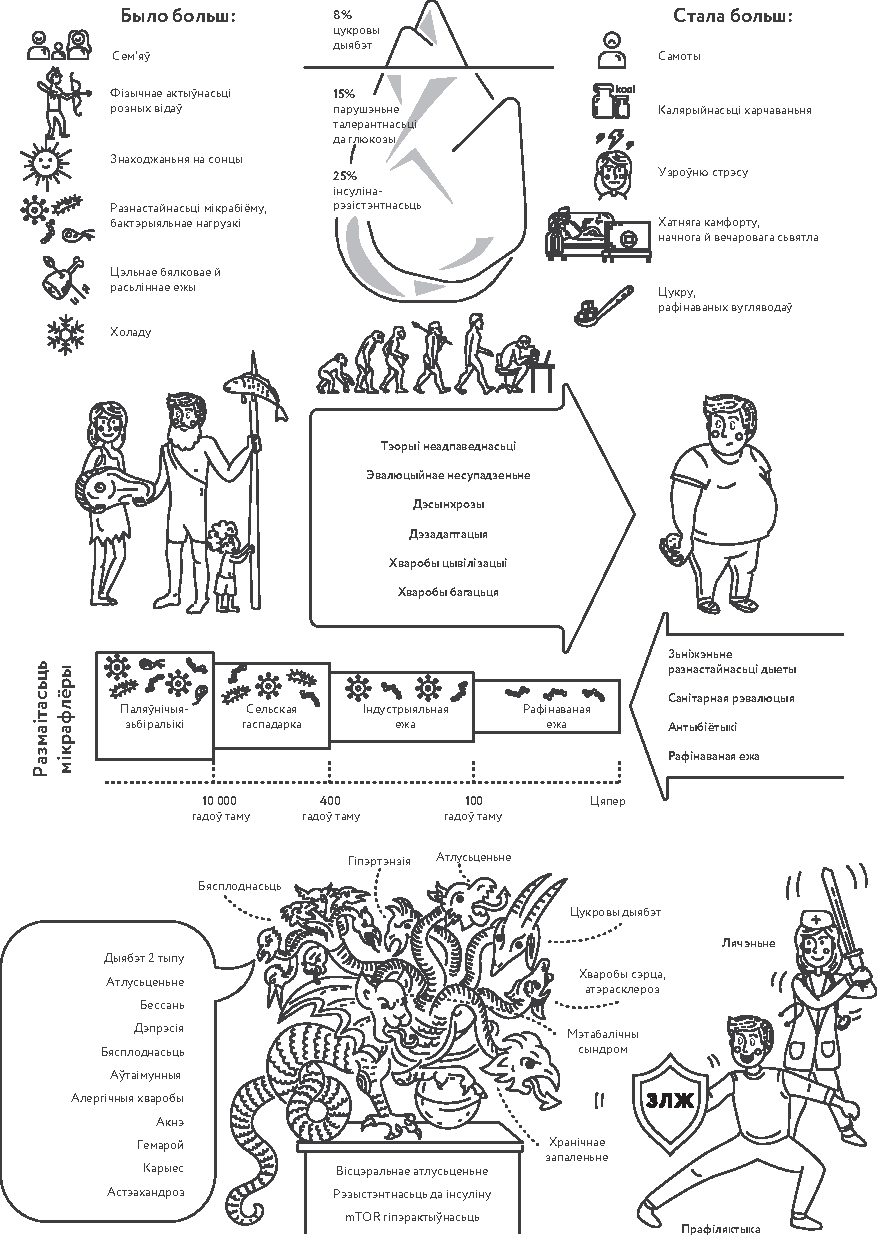
\includegraphics[width=\textwidth]{willpower/ch2/full.pdf}  
\end{figure*}

